% Tipo de documento
\documentclass[12pt,a4paper]{article}

% Pacotes
%\usepackage{showlabels}
\usepackage{latexsym}
\usepackage{amsfonts}
\usepackage{amsmath}
\usepackage{amscd}
\usepackage[brazil]{babel}
\usepackage[utf8]{inputenc}
\usepackage[pdftex]{graphicx}
\usepackage{multirow}

% Paginação
%\textwidth 15.0cm                    % Largura
%\textheight 22.0cm                   % Altura
%\addtolength{\oddsidemargin}{0.0cm}  % Margem esquerda (impar)
%\addtolength{\evensidemargin}{0.0cm} % Margem esquerda (par)
%\addtolength{\topmargin}{0.0cm}      % Margem superior

% Estilo dos parágrafos
\sloppy                              % Mais flexível
\setlength{\jot}{08pt}               % Distância entre linhas do eqnarray
\setlength{\parskip}{1ex}            % Distância entre parágrafos
\renewcommand{\baselinestretch}{1.0} % Distância entre linhas

% Comandos customizados
\newcommand{\vet}{\mathbf}                                   % vetor
\newcommand{\ie}{\emph{i.e.}}                                % isto é
\newcommand{\prodint}[2]{\left\langle #1 , #2 \right\rangle} % produto interno
\newcommand{\Fullbox}{{\rule{2.0mm}{2.0mm}}}                 % caixa cheia
\newcommand{\EOS}{\hfill\Box\vspace{-0.2cm}}                 % fim de enunciado
\newcommand{\EOP}{\hfill\Fullbox\vspace{0.2cm}}              % fim de prova
\newcommand{\eps}{\varepsilon}                               % epsilon
\newcommand{\defi}{\: := \: }                                % definição
\newcommand{\del}{\partial}                                  % derivada parcial
\newcommand{\hsp}{\hspace{0.5cm}}                            % espaco horizontal para fórmulas
\newcommand{\vsp}{\vspace{0.1cm}}                            % espaco vertical para fórmulas
\newcommand{\ev}{\, ,}                                       % espaco e virgula
\newcommand{\ep}{\, .}                                       % espaco e ponto
\newcommand{\eg}{\emph{e.g.}}                               % por exemplo

% Fontes caligráficas
\newcommand{\calA}{\mathcal{A}} 
\newcommand{\calC}{\mathcal{C}}
\newcommand{\calR}{\mathcal{R}}                             

% Contagem de equações por seção
\renewcommand{\theequation}{\thesection.\arabic{equation}}

% Contagem de figuras por seção
\renewcommand{\thefigure}{\thesection.\arabic{figure}}

% Contagem de tabelas por seção
\renewcommand{\thetable}{\thesection.\arabic{table}}

% Zerar as contagem em cada seção
\newcommand{\zerar}{\setcounter{equation}{0}\setcounter{figure}{0}\setcounter{table}{0}}

% Operadores
\DeclareMathOperator{\sen}{sen}
\DeclareMathOperator{\tg}{tg}
\DeclareMathOperator{\cotg}{cotg}
\DeclareMathOperator{\im}{im}
\DeclareMathOperator{\arctg}{arctg}
\DeclareMathOperator{\diag}{diag}
\DeclareMathOperator{\sgn}{sgn}
\DeclareMathOperator{\tr}{tr}

% Conjunto de números
\newcommand{\Z}{\mathbb{Z}}
\newcommand{\C}{\mathbb{C}}
\newcommand{\N}{\mathbb{N}}
\newcommand{\Q}{\mathbb{Q}}
\newcommand{\R}{\mathbb{R}}

%%%%%%%%%%%%%%%%%%%%%%%%%%%%%%%%%%%%%%%%%%%%%%%%%%%%%%%%%%%%%%%%%%%%%%%%%%%%%%%%%%%%%%%%%%%%%%%%%%%%

\begin{document}

\title{\bf Otimização do Escalonamento de Tripulantes em Companhias Aéreas}
\author{Daniel Augusto Cortez \\ Lucas Rodrigues Colucci \\ Renato Lerac Corrêa de Sá}
\date{\today}

\maketitle

\begin{abstract}
	Versão preliminar da monografia a ser apresentada como trabalho de conclusão de curso. Contém
	uma introdução ao problema, a análise preliminar, alguns resultados obtidos até o momento e 
	conclusões.
\end{abstract}

\vspace{1cm}

\begin{center}
	{\bf Orientador:} Alfredo Goldman Vel Lejbman

	\vspace{1.5cm}

	{\bf Blog:} \verb|http://social.stoa.usp.br/profile/daniel-lucas-renato|

	{\bf GitHub:} \verb|https://github.com/bublecamp/TCC2012| 
\end{center}

\thispagestyle{empty}

\newpage 

\tableofcontents

\newpage

%%%%%%%%%%%%%%%%%%%%%%%%%%%%%%%%%%%%%%%%%%%%%%%%%%%%%%%%%%%%%%%%%%%%%%%%%%%%%%%%%%%%%%%%%%%%%%%%%%%%

\zerar
\section{Introdução}
\label{sec:introducao}

Métodos de otimização no planejamento das operações de uma empresa aérea têm sido aplicados a várias
décadas~\cite{yu}. Tal planejamento envolve diversos problemas que normalmente são resolvidos de
forma separada e sequencial devido ao tamanho e a complexibilidade de cada problema individual,
embora eles estejam intimamente relacionados~\cite{barnhart03} (veja Figura~\ref{fig:planejamento}).

Primeiro, resolve-se o problema da \emph{malha de voos}, que consiste em determinar todos os trechos
a serem voados pela empresa num determinado período de tempo. O planejamento é basicamente feito em
termos de demanda de mercado.

Segundo, trata-se do problema da \emph{atribuição de frotas}. Nele, determina-se qual o tipo de
aeronave (tal como Boeing 737, Boeing 767, Airbus 320, etc) deve ser atribuído para efetuar cada
trecho da malha de voos. O objetivo é maximizar os lucros de venda, em função da demanda prevista e
do custo de se operar determinada frota em determinado trecho, sujeito à restrição de que todos os
voos da malha sejam cobertos com a frota disponível.

Terceiro, considera-se o problema do \emph{roteamento de aeronaves}, que envolve a escolha das
aeronaves de uma frota que vão realizar determinados voos de forma que cada aeronave passe um tempo
adequado em aeroportos específicos com a finalidade de serem revisadas pela manutenção. O objetivo é
maximizar os lucros, respeitando ainda a restrição de que todos os voos da frota sejam cobertos.

Finalmente, o problema de \emph{escalonamento de tripulantes} é resolvido. Tal problema foi um dos
primeiros a receber atenção significativa por parte da comunidade de pesquisa
operacional~\cite{arabeyre69}, sendo ainda um dos mais estudados. Isso porque, no transporte aéreo,
os custos com a tripulação representam a segunda maior parcela dos custos operacionais da empresa,
perdendo apenas para os custos com combustível. Para se ter uma ideia, o custo total com tripulação
excede 1,3 bilhões de dólares todo ano na Americam Airlines~\cite{anbil91a}. Hoje em dia, a
otimização no planejamento de escalas representa economia de cerca de 50 milhões de dólares anuais
para uma companhia de grande porte~\cite{barnhart03}.

\begin{figure}[htbp]
	\begin{center}
		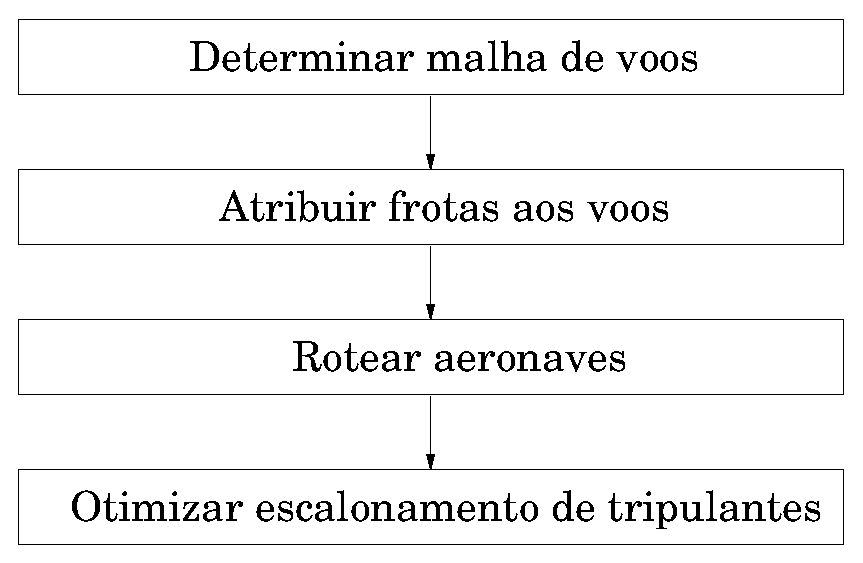
\includegraphics[scale=0.5]{fig/planejamento.eps}
		\caption{Sequência de problemas resolvidos no planejamento de operações de uma empresa aérea.}
		\label{fig:planejamento}
	\end{center}
\end{figure}

De forma geral, escalonamento de tripulantes pode ser definido como o problema de se atribuir um
grupo de trabalhadores (uma tripulação) para realizar um conjunto de atividades. No contexto da
aviação, cada tripulante (comandante, co-piloto, comissário, etc) deve ser designado para realizar
um determinado voo da empresa. Tal designação deve ser feita respeitando-se uma série de restrições
impostas pelas agências reguladoras da aviação, bem como regras de regulamentação trabalhista,
restrições operacionais impostas pela própria empresa e acordos trabalhistas entre empregado e
empregador. Dado o grande número de variáveis e restrições envolvidas, assim como a possibilidade de
grandes ganhos econômicos, o problema torna-se bastante interessante, tanto do ponto de vista da
indústria, quanto acadêmico.

Neste trabalho focaremos justamente na parte de escalonamento de tripulantes, mais especificamente
no chamado problema da determinação das viagens. O objetivo é apresentar, discutir e implementar 
alguns dos métodos de solução disponíveis na literatura, apresentando alguns resultados no contexto
das companhias aéreas brasileiras.

%%%%%%%%%%%%%%%%%%%%%%%%%%%%%%%%%%%%%%%%%%%%%%%%%%%%%%%%%%%%%%%%%%%%%%%%%%%%%%%%%%%%%%%%%%%%%%%%%%%%

\subsection{Definições e Nomenclaturas}
\label{sec:definicoes}

Antes que possamos apresentar e explorar a estrutura do problema com mais detalhes, faz-se
necessário a introdução de algumas definições e nomenclaturas normalmente utilizadas, as quais serão
amplamente utilizadas neste trabalho.

\begin{itemize}
	\item {\bf Etapa:} é um voo único sem paradas, também chamado de {\bf perna}, {\bf trecho} ou {\bf 
	segmento de voo}.
	\item {\bf Jornada:} conjunto de uma ou mais etapas sequenciais, também chamado de {\bf jornada 
	de trabalho}. 
	\item {\bf Tempo Mínimo de Conexão:} menor intervalo possível de tempo entre duas etapas 
	consecutivas em uma jornada.
	\item {\bf Tempo Máximo de Conexão:} maior intervalo possível de tempo entre duas etapas 
	consecutivos em uma jornada.
	\item {\bf Tempo de Briefing:} tempo mínimo que antecede o início da primeira etapa de uma
	jornada, necessário para o {\it briefing} da tripulação.
	\item {\bf Tempo de Debriefing:} tempo mínimo que sucede o término da último etapa de uma jornada,
	necessário para o {\it debriefing} da tripulação.
	\item {\bf Início da Jornada:} horário em que a tripulação deve se apresentar para o início de
	uma jornada. Corresponde ao horário da decolagem da primeira etapa menos o tempo de 
	{\it briefing}. 
	Também chamado de {\bf checkin}.
	\item {\bf Término da Jornada:} horário em que a tripulação encerra suas atividade em uma 
	jornada. Corresponde ao horário de pouso da última etapa mais o tempo de {\it debriefing}.
	Também chamado de {\bf checkout}.
	\item {\bf Base Contratual:} cidade onde uma dado tripulante está domiciliado, também chamada 
	simplesmente de {\bf base}.
	\item {\bf Viagem:} conjunto de jornadas de trabalho, com a primeiro etapa da primeira jornada e
	a última etapa da última jornada começando e terminando na mesma base contratual. 
	Uma viagem também é chamada de {\bf pairing}, ou {\bf rotação}.
	\item {\bf Descanso:} intervalo mínimo de tempo ininterrupto de repouso após uma jornada.
	\item {\bf Pernoite:} intervalo de tempo separando duas jornadas consecutivas de uma viagem.
	\item {\bf Reserva:} período de tempo em que o tripulante permanece, por determinação do 
	empregador, em local de trabalho à sua disposição.
	\item {\bf Sobreaviso:} período de tempo não excedente a 12 horas, em que o tripulante permanece 
	em local de sua escolha, à disposição do empregador, devendo apresentar-se em até 90 minutos após 
	receber comunicação para o início de nova tarefa.
	\item {\bf Folga:} período de tempo não inferior a 24 horas consecutivas em que o tripulante, em 
	sua base contratual, sem prejuízo de remuneração, está desobrigado de qualquer atividade
	relacionada com seu trabalho.
	\item {\bf Escala:} conjunto de viagens, reservas, sobreavisos, folgas e deveres extra-voo
	(cursos, treinamentos em simulador, férias, etc), expandindo um determinado horizonte de tempo, 
	que definem as atividades de um tripulante. 
\end{itemize}

A Figura~\ref{fig:viagem} apresenta o exemplo de uma viagem que ilustra alguns dos conceitos
expostos acima. As etapas na figura estão representadas pelos retângulos mais internos. São
indicados os aeroportos de origem e destino, bem como os horários de decolagem e pouso. As
jornadas são indicadas pelos retângulos pontilhados, englobando uma cadeia de etapas. A base 
contratual considerada é CGH (São Paulo). 

\begin{figure}[htbp]
	\begin{center}
		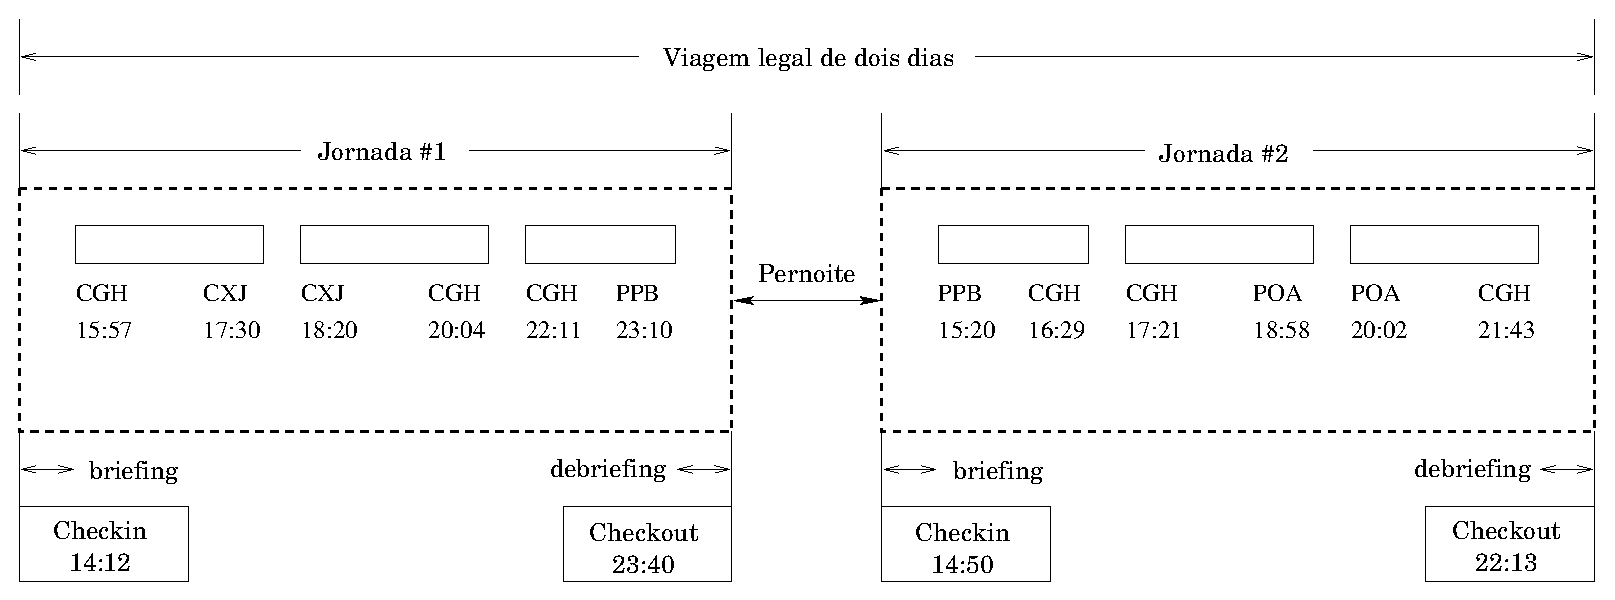
\includegraphics[scale=0.5]{fig/viagem.eps}
		\caption{Exemplo de uma viagem de dois dias para a base CGH.}
		\label{fig:viagem}
	\end{center}
\end{figure}

A Figura~\ref{fig:escala} apresenta o exemplo de uma escala de um determinado tripulante. O 
horizonte de tempo considerado é de 15 dias. Para fins de ilustração, foram alocadas três 
viagens viagens (c), (a) e (b) nos dias 3, 5--8 e 12--14, respectivamente. Os demais dias foram 
preenchidos com períodos de folgas, sobreaviso, reserva e um curso.

\begin{figure}[htbp]
	\begin{center}
		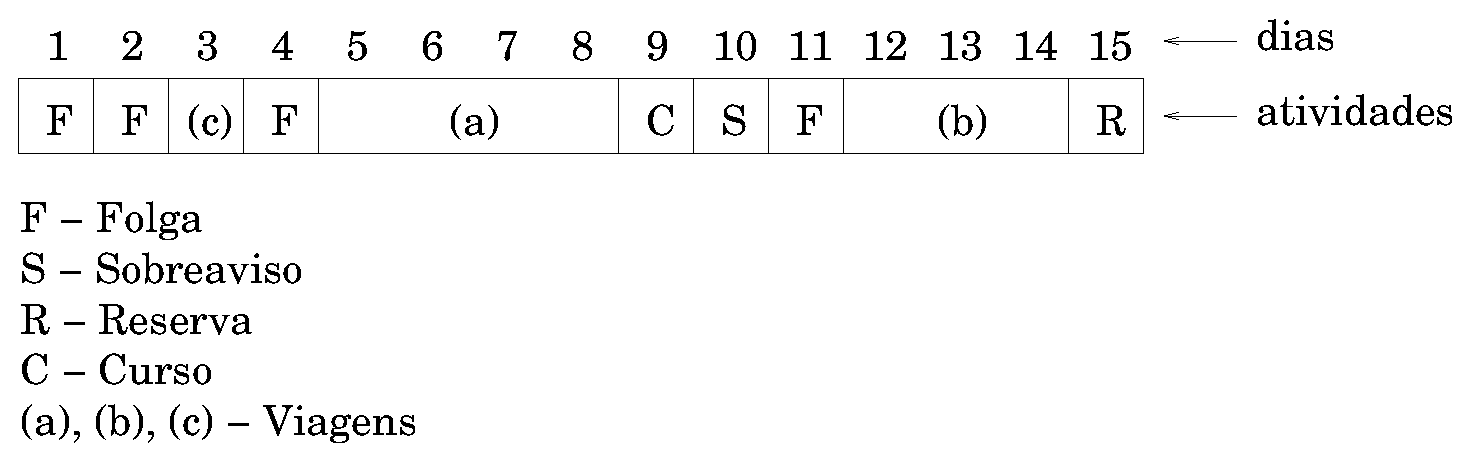
\includegraphics[scale=0.5]{fig/escala.eps}
		\caption{Exemplo de uma escala com diversas atividades para um dado tripulante.}
		\label{fig:escala}
	\end{center}
\end{figure}

%%%%%%%%%%%%%%%%%%%%%%%%%%%%%%%%%%%%%%%%%%%%%%%%%%%%%%%%%%%%%%%%%%%%%%%%%%%%%%%%%%%%%%%%%%%%%%%%%%%%

\zerar
\section{Formulação do Problema}
\label{sec:formulacao}

Normalmente o problema do escalonamento de tripulantes é dividido em dois subproblemas que são
resolvidos de forma independente e sequencial. O primeiro deles é conhecido como \emph{problema da
determinação de viagens} (PDV), que consiste na obtenção de um subconjunto de viagens, obedecendo as
regras de trabalho impostas pela legislação, com custo mínimo, cobrindo todas os segmentos de voo
exatamente uma vez. Obtida a solução das viagens, um segundo problema é resolvido, conhecido como
\emph{problema da determinação de escalas} (PDE), cujo objetivo é construir as escalas dos
tripulantes, distribuindo as viagens de tal forma que cada viagem seja atribuída exatamente uma vez
para cada tripulante requerido. Na atribuição, visa-se minimizar os custos e garantir distribuição
uniforme de trabalho. A atribuição das viagens também está sujeita a uma série restrições
reguladoras.

Tanto o PDV quanto o PDE têm sido extensamente estudados na literatura~\cite{gopalakrishnan05}. Em
especial, o primeiro deles recebeu mais atenção, principalmente no contexto norte-americano, dada o
seu potencial em produzir economia significativa de custos. No problema da determinação de escalas,
além de minimizar custos, é importante também levar em conta aspectos da qualidade de vida dos
tripulantes. Uma visão geral e esquemática dos dois problemas é apresentada na
Figura~\ref{fig:escalonamento}.

As modelagens matemáticas usuais do PDV e do PDE são semelhantes e baseiam-se em um problema de 
programação linear inteiro conhecido como \emph{set partition problem}. A técnica de resolução comum 
utilizada pode ser descrita como ``gerar-e-otimizar''. Outras abordagens vem sendo recentemente 
propostas, buscando por soluções através de métodos meta-heurísticos. Nas próximas seções 
apresentaremos mais detalhes sobre as duas abordagens.

\begin{figure}[htbp]
	\begin{center}
		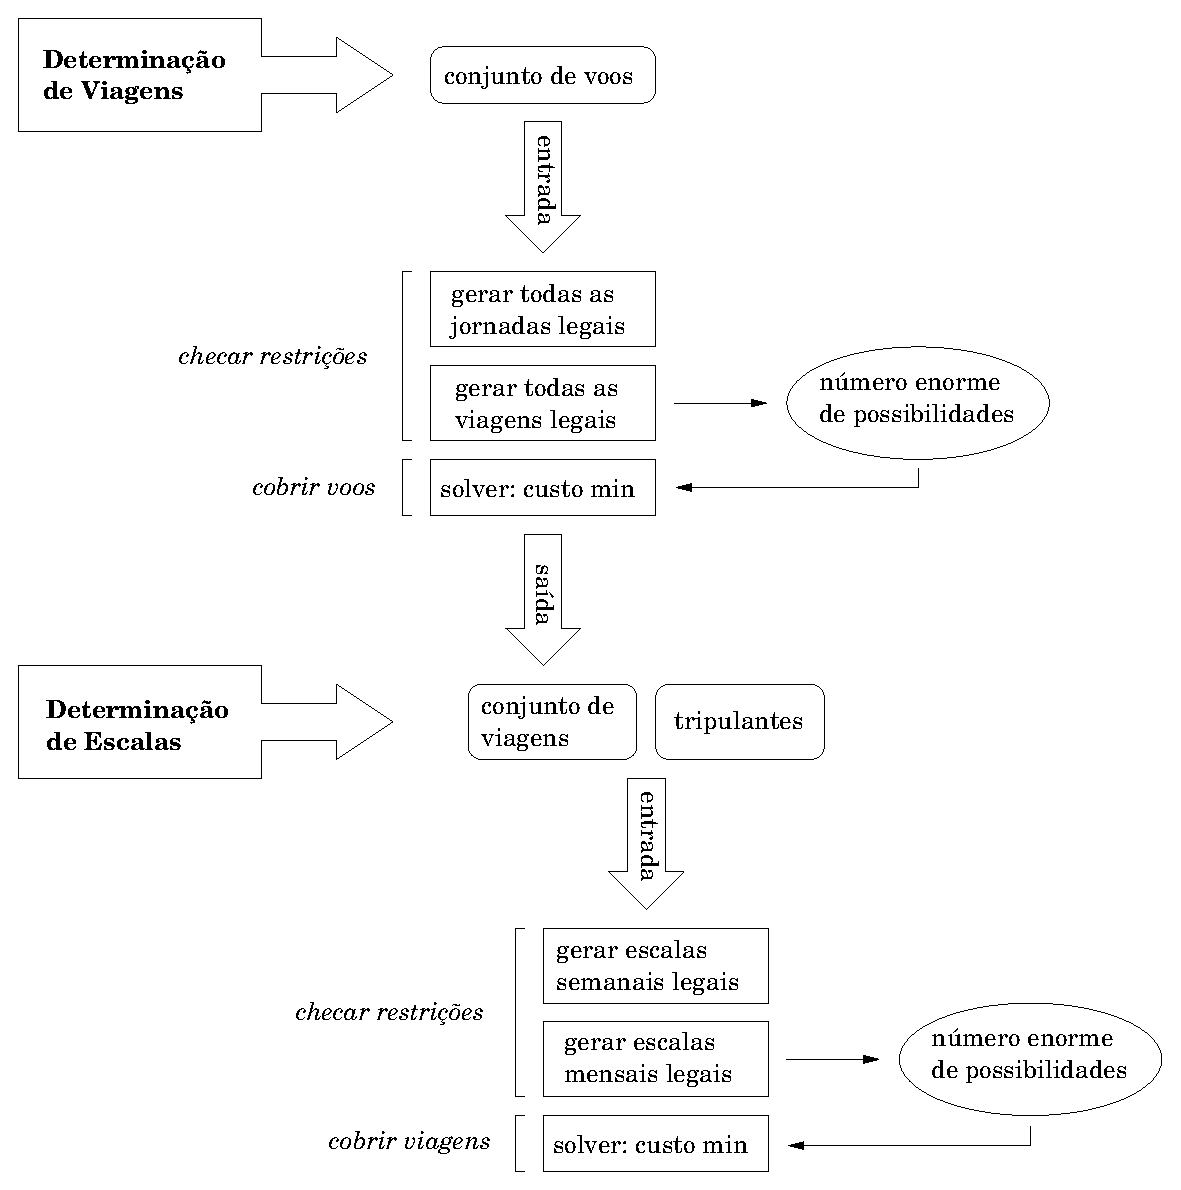
\includegraphics[scale=0.6]{fig/escalonamento.eps}
		\caption{Subproblemas enfrentados na solução do problema de escalonamento de tripulantes 
		(adaptado de~\cite{souai09}).}
		\label{fig:escalonamento}
	\end{center}
\end{figure}

\subsection{Regras de Trabalho e Estrutura de Custo}
\label{sec:regras_e_custos}

Antes de entrarmos nos detalhes sobre a formulação do PDV e do PDE, é interessante explicitar os 
tipos de restrições e a estrutura de custo envolvidos nos problemas, em especial no contexto 
brasileiro, já que há uma diferença significativa com relação aos contextos norte-americano e 
europeu, normalmente analisados na literatura.

No caso do PDV, a geração de uma viagem é regida por uma série de regras impostas pela Agência
Nacional de Aviação Civil (ANAC), além de restrições impostas por leis trabalhistas e acordos
contratuais. Uma viagem é dita legal se ela obedecer todas as regras impostas pela legislação em
questão. Abaixo apresenta-se valores típicos para as regras que regem a construção de uma viagem em
uma empresa de aviação regular do Brasil com voos de curto e médio alcance:

\begin{itemize}
	\item Duração máxima de uma jornada de trabalho: 11 horas;
	\item Número máximo de horas de voo em uma jornada: 9 horas e 30 minutos;
	\item Número máximo de pousos em uma jornada: 6 pousos;
	\item Descanso mínimo entre jornadas: 12 horas;
	\item Tamanho máximo de uma viagem: 6 dias;
	\item Tempo mínimo de conexão: 30 minutos;
	\item Tempo máximo de conexão: 4 horas;
	\item Número máximo de trocas de aeronave em uma jornada: 2 trocas;
	\item Tempo de briefing: 30 minutos fora de base e 45 minutos dentro;
	\item Tempo de debriefing: 30 minutos.
\end{itemize}

O custo de uma viagem está associado à produtividade mais os custos referentes à estadia do 
tripulante quando esse precisar pernoitar fora da base, além das diárias de alimentação. Uma 
expressão típica para calcular o custo $c_p$ de uma viagem $p$ é dada por
%
\begin{equation} \label{eq:custov} 
	c_p = \sum_{d \in D_p} c_d \, , \;\;
	c_d = \alpha_0 \left[t_d - \left(tp_d - \sum_{i \in I_d} t_i\right)\right] + cp_d \ev
\end{equation} 
%
onde
%
\begin{itemize}
	\item[$D_p$:] conjunto de jornadas que constituem a viagem $p$;
	\item[$c_d$:] custo da jornada $d$;
	\item[$\alpha_0$:] custo da hora de trabalho do tripulante;
	\item[$t_d$:] duração da jornada $d$ (em horas);	
	\item[$tp_d$:] tempo de preparação ({\it briefing} mais {\it debriefing}) usado na jornada $d$;
	\item[$I_d$:] conjunto de etapas que compõe a jornada $d$;
	\item[$t_i$:] duração da etapa $i$, incluindo o tempo mínimo de conexão;
	\item[$cp_d$:] custo do pernoite mais diárias de alimentação da jornada $d$.
\end{itemize}
%
Note que a expressão que multiplica $\alpha_0$ em (\ref{eq:custov}) representa o tempo que o
tripulante passou trabalhando sem estar voando, portanto representa uma medida de produtividade.
Quanto mais cara a viagem, menor foi a produtividade do tripulante.

No PDE também aplica-se uma série de regras trabalhistas para geração de uma escala legal. Dentre 
elas, podemos citar como mais importantes:

\begin{itemize}
	\item Número mínimo de folgas: 8 folgas, sendo no mínimo 2 em um final de semana;
	\item Intervalo máximo de trabalho sem folgas: 6 dias;
	\item Número máximo de horas de voo em um mês: 85 horas;
	\item Número máximo de horas de uma reserva: 6 horas;
	\item Número máximo de sobreavisos: 2 semanais e 8 mensais.
\end{itemize}

O custo associado a uma dada escala legal montada para um tripulante é bastante dependente da
política de pagamento da empresa. No Brasil, em geral, as companhias costumam pagar um salário fixo
e mais um excedente por hora voada se o número de horas voadas pelo tripulante extrapolar um
determinado valor. Além disso, horas voadas no período noturno, domingos e feriados, chamadas horas
especiais, são pagas a partir do zero. Assim, podemos calcular o custo $c_k$ de uma escala atribuída
a um tripulante $k$ como
%
\begin{equation*}
c_k = \alpha_1 + \alpha_2 \sum_{p \in P_k} e_p 
	+ \alpha_3 \max\left\{0, \left(\sum_{p \in P_k} t_p\right) - mg\right\}
	+ \sum_{p \in P_k} c_p \ev
\end{equation*}
%
onde
%
\begin{itemize}
	\item[$\alpha_1$:] remuneração fixa do tripulante;
	\item[$\alpha_2$:] remuneração por cada hora especial realizada;
	\item[$\alpha_3$:] remuneração por cada hora de voo excedente à garantia mínima;
	\item[$P_k$:] conjunto de viagens atribuídas ao tripulante $k$;	
	\item[$e_p$:] horas de voo especiais na viagem $p$;
	\item[$t_p$:] horas de voo na viagem $p$;
	\item[$mg$:] garantia mínima de horas de voo;
	\item[$c_p$:] custo da viagem $p$.
\end{itemize}
%
Note que consideramos apenas a atribuição de viagens na escala de tripulantes. Atividades de reserva
e sobreaviso também entram na remuneração contando como se fossem horas de voo. No caso do
sobreaviso, o valor deve ser multiplicado por $1/3$.

A estrutura descrita acima se refere a um modelo padrão para companhias aéreas brasileiras.
Fora do Brasil, entretanto, a estrutura do custos pode ser diferente. Nos Estados Unidos, por 
exemplo, o custo de uma viagem é dado por uma função não-linear de diferentes custos. 
Especificamente, o custo de uma viagem $p$ é dado por
%
\begin{equation*}
	c_p = \max\left\{\sum_{d \in D_p} MIN\_GRT_d \ev \sum_{d \in D_p} FLY\_TIME_d \ev 
	TIME\_AWAY_p \right\} \ev
\end{equation*}
%
onde $MIN\_GRT_d$ é o mínimo de garantia oferecido ao tripulante ao voar a jornada $d$, 
$FLY\_TIME_d$ é o tempo de voo da jornada $d$ (pode ser multiplicado por algum fator) e
$TIME\_AWAY_p$ é o tempo total que o tripulante passa fora de sua base na viagem $p$ (também pode
ser multiplicado por algum fator). Observe assim, que nesse modelo, o custo de cada etapa depende da
viagem em ela está incluída.

%%%%%%%%%%%%%%%%%%%%%%%%%%%%%%%%%%%%%%%%%%%%%%%%%%%%%%%%%%%%%%%%%%%%%%%%%%%%%%%%%%%%%%%%%%%%%%%%%%%%

\subsection{Problema da Determinação das Viagens}
\label{sec:viagens}

No problema da determinação das viagens, tem-se como entrada o conjunto de voos a ser operado pela
empresa, o conjunto de bases contratuais dos tripulantes, as regras de trabalho que ditam a
construção de viagens legais e a estrutura de custo como descrita na equação (\ref{eq:custov}). A
saída então deve ser um conjunto de viagens que cubra todos os voos operados exatamente e uma vez e
que gere o custo mínimo (veja Figura~\ref{fig:pdv}).

\begin{figure}[htbp]
	\begin{center}
		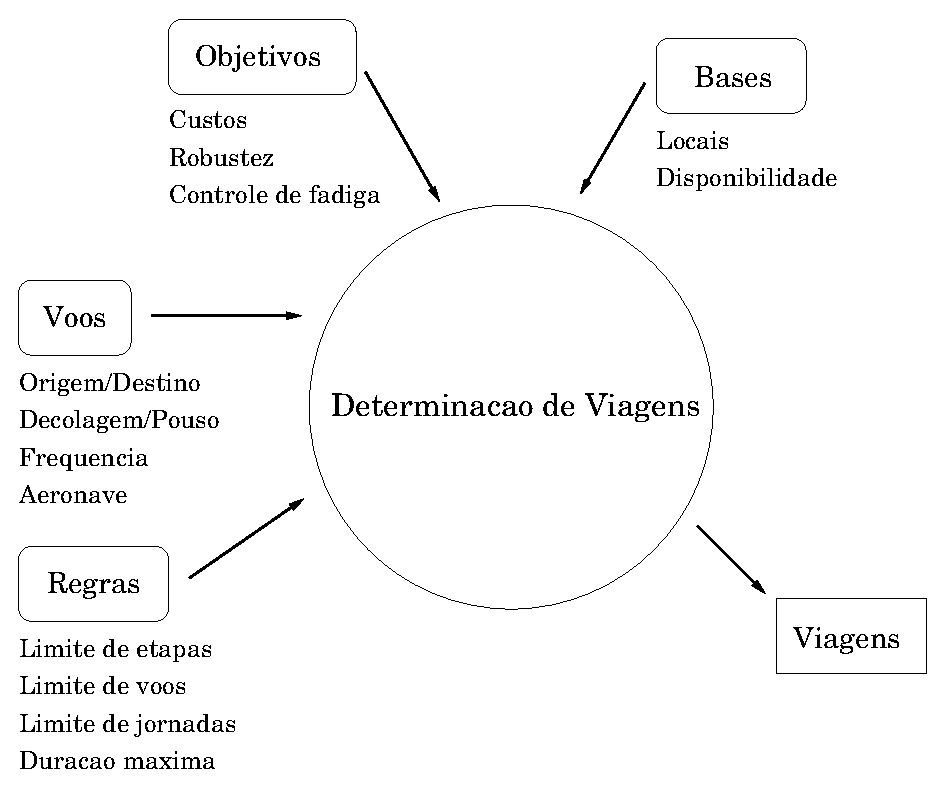
\includegraphics[scale=0.5]{fig/pdv.eps}
		\caption{Representação do problema da determinação de viagens (PDV).}
		\label{fig:pdv}
	\end{center}
\end{figure}

Normalmente os voos das companhias aéreas apresentam uma frequência regular de oferecimento, sendo
que a maioria deles operam diariamente. Outros são oferecidos apenas em alguns dias fixos da semana
e poucos são oferecidos vez ou outra no mês. Costuma-se então inicialmente resolver o problema
diário, onde se assume que todos os voos são repetidos diariamente. Note que para o problema diário,
viagens de vários dias com etapas repetidas são inviáveis. Um segmento de voo repetido causaria o
efeito de mais de uma tripulação ser atribuída para realização dessa etapa, uma vez que quando se
faz a implementação da solução diária, uma tripulação distinta é atribuída a cada um dos dias da
viagem.

O problema semanal é mais complicado porque envolve um maior número de etapas consideradas. De
qualquer forma, a solução do problema semanal pode ser obtido a partir de um ajuste da solução do
problema diário, sem perda significativa de custo~\cite{gopalakrishnan05}. A solução do problema
mensal completo segue da solução do problema semanal. Como a maior parte da redução de custos está
associada à resolução do problema diário, ele se torna o mais importante. Daqui em diante trataremos
apenas do problema diário.

Uma outra simplificação do problema está no fato que os tripulantes são habilitados para operar
apenas um tipo, ou família, de aeronaves dentro de uma frota. Assim, fatora-se o problema da
determinação das viagens por tipo de aeronave. Para cada tipo, resolve-se um PDV considerando apenas
as etapas operadas por aquele tipo. As viagens assim geradas são atribuídas aos tripulantes
habilitados no tipo ao se resolver o PDE.

Há uma formulação natural para o PDV em termos de um problema de programação linear. Suponha que
seja possível gerar e enumerar todas as $n$ viagens associadas a uma dada entrada do problema
contendo $m$ etapas a serem cobertas. Seja $x_j \in \{0, 1\}$ uma variável de decisão que assume o
valor 1 se a viagem $j$ for escolhida na solução de custo mínimo e 0 caso contrário. Então, o PDV
pode ser modelado da seguinte forma:
%
\begin{eqnarray} \label{eq:sppv}
	\text{minimizar} && \displaystyle \sum_{j=1}^n c_j x_j \nonumber \\
	\text{sujeito à} && \displaystyle \sum_{j=1}^n a_{ij} x_j = 1 \ev \;\; i = 1, \ldots, m \\
		               && x_j \in \{0, 1\} \ev \;\; j = 1, \ldots, n \ep \nonumber
\end{eqnarray} 
%
Os coeficientes $a_{ij}$ são definidos por
%
\begin{equation*}
	a_{ij} = \left\{
	\begin{array}{ll}
			1 \ev & \text{se a viagem $j$ cobre a etapa $i$} \\
			0 \ev & \text{caso contrário}
	\end{array}
	\right.
\end{equation*}

As restrições em (\ref{eq:sppv}) garantem que cada etapa seja coberta exatamente uma vez por alguma
viagem. Existe ainda uma formulação alternativa onde as restrições são dadas por
%
\begin{equation} \label{eq:dh} 
	\sum_{j=1}^n a_{ij} x_j \geq 1 \, , \;\; i = 1, \ldots, m \ep
\end{equation} 
%
Nesse caso uma mesma etapa pode ser coberta por mais de uma viagem e o problema se torna um
\emph{set cover problem}. Do ponto de vista do escalonamento, se uma etapa é coberta por mais
de uma viagem, então uma tripulação estará trabalhando nessa etapa e as demais viajando de
passageiro (situação conhecida por \emph{deadheading}). As vezes essa formulação é necessária para
que se garanta viabilidade da solução. Se o preço a se pagar pela operação com \emph{deadheading} 
for essencialmente o mesmo de uma operação normal, então não há alteração significativa no custo 
da viagem associada. Isso permite que o problema seja modelado com as restrições (\ref{eq:dh}) 
sem alterar a estrutura de custos.

É comum a inserção de restrições adicionais ao modelo que garantem uma distribuição de trabalho
entre as bases compatível com os recursos disponíveis em cada base. Se o número total de bases do
problema considerado é $r$, então as \emph{restrições de bases} são expressas por
%
\begin{equation} \label{eq:bases}
	H_k^L \leq \sum_{j=1}^n h_{kj} x_j \leq H_k^U \, , \;\; k = 1, \ldots, r \ev
\end{equation}
%
onde $H_k^L$ é o número mínimo de horas disponíveis na base $k$ e $H_k^U$ é seu número máximo. 
Note que $H_k^L$ pode ser diferente de zero desde que se exija que não mais do que um certo número 
de tripulantes fiquem de reserva. O coeficiente $h_{kj}$ dá o número de horas necessárias para 
efetuar a viagem $j$ ($h_{kj} = 0$ se a viagem $j$ não pertencer à base $k$).

O grande problema com a formulação (\ref{eq:sppv}) está no enorme número de variáveis geradas mesmo
nos casos das instâncias pequenas (poucas etapas diárias). A Tabela~\ref{tab:viagens} ilustra o
número de viagens legais geradas, com duração máxima de 3 ou 4 dias, para diversas frotas de
aeronaves. O número enorme de variáveis está associada com a natureza combinatória do problema. A
maioria das empresas aéreas operam em aeroportos conhecidos como \emph{hubs}, onde um grande número
de aeronaves chegam e partem em um mesmo intervalo de tempo, possibilitando que os passageiros
efetuem suas conexões para uma grande quantidade de destinos em pouco tempo. Esse tipo de estrutura
em rede leva à explosão no número de viagens legais que podem ser construídas~\cite{graves93}.
Note da Tabela~\ref{tab:viagens} que apesar do número de viagens ser gigantesco, o número de 
jornadas tem um valor muito mais gerenciável.

\begin{table}[ht]
	\begin{center}
		\begin{tabular}{|c||c|c|c|c|c|}
			\hline
			{\bf Frota} & {\bf Max Dias} & {\bf Etapas} & {\bf Bases} & {\bf Jornadas} & 
			{\bf Viagens} ($\times 10^6$) \\
			\hline
			AAS80 & 3 & 1.152 & 12 & 690.000 & 48.400 \\
			\hline
			AA757 & 3 & 251 & 15 & 7.000 & 1 \\
			\hline
			AA727 & 3 & 375 & 11 & 31.000 & 36 \\
			\hline
			AAF10 & 4 & 307 & 3 & 55.000 & 63.200 \\
			\hline 
			UA737 & 4 & 773 & 7 & 568.000 & 100.000.000 \\
			\hline
			USDC9 & 4 & 478 & 4 & 562.000 & 105.000.000 \\
			\hline
		\end{tabular}
		\caption{Jornadas e viagens legais geradas para um conjunto de frotas de aeronaves de companhias
		norte-americanas (fonte:~\cite{anbil98}).}
		\label{tab:viagens}
	\end{center}
\end{table}

Como o problema de partição é do tipo NP-difícil, a aplicação de métodos diretos de otimização é
impraticável para qualquer situação real. Discutiremos esse ponto na Seção~\ref{sec:analise_p}. Os
métodos de solução normalmente envolvem algum tipo de heurística e/ou algum critério de parada que
leva a soluções sub-ótimas.

%%%%%%%%%%%%%%%%%%%%%%%%%%%%%%%%%%%%%%%%%%%%%%%%%%%%%%%%%%%%%%%%%%%%%%%%%%%%%%%%%%%%%%%%%%%%%%%%%%%%

\subsubsection{Gerador de Viagens}
\label{sec:gerador_viagens}

O primeiro passo em direção à solução do PDV consiste na implementação de um gerador de viagens 
eficiente que seja capaz de produzir um grande número de viagens legais em pouco tempo. Como já
mencionamos, os métodos de resolução de (\ref{eq:sppv}) baseiam-se no conceito de 
``gerar-e-otimizar'', e já que as rotinas de otimização estão normalmente prontas em pacotes 
fechados, a parte de geração é de grande importância.

Uma viagem pode ser vista como um caminho especial em um grafo estruturado. Esse grafo é chamado de
\emph{rede de voos} e será detalhado a seguir. 

As etapas na rede de voos podem ser representadas como nós ou arcos. Escolhemos a representação em
termos de arcos. Os nós da rede representam as saídas e chegadas de cada etapa, bem como uma fonte
$s$ e um sorvedouro $t$. Existe um arco representando cada etapa da malha de voos. Para o problema
diário, replicamos cada arco quantas vezes for o número máximo de dias permitido em um viagem. O
conjunto de arcos será denotado por $\calA$.

O nó fonte é ligado ao nó de saída de cada etapa que se origina em uma base específica. O nó de
chegada de cada etapa que termina nessa base é ligado ao sorvedouro. Existem ainda arcos
representando conexões legais entre etapas. Um par de etapas terá um arco de conexão entre eles se
o aeroporto de chegada do primeiro corresponder ao aeroporto de saída do segundo, e o intervalo de
tempo entre a chegada e a saída estiver for uma conexão legal de uma jornada, 
ou descanso regular entre jornadas. 

É fácil notar que toda viagem legal é representada por um caminho $s-t$ na rede de voos. Porém,
existem caminhos $s-t$ que não representam viagens legais pois podem desrespeitar alguma regra de
trabalho, embora as conexões possíveis sejam legais. A estrutura da rede garante que não seja feita
nenhuma conexão entre duas etapas que não tenham suas respectivos destino e origem coincidentes no
espaço e no tempo. Entretanto, não garante, por exemplo, que o número máximo de horas de voo
permitido em uma jornada seja excedido. 

O gerador de viagens funciona aplicando um algoritmo de busca em profundidade à rede de voos. O
algoritmo inicia-se no nó de origem $s$ e explora todas a conexões viáveis $(i, j) \in \calA$, até
retroceder. O processo de busca em profundidade controla a viabilidade das viagens, levando em conta
a duração máxima das jornadas e limites de horas de voo e de pousos.

%%%%%%%%%%%%%%%%%%%%%%%%%%%%%%%%%%%%%%%%%%%%%%%%%%%%%%%%%%%%%%%%%%%%%%%%%%%%%%%%%%%%%%%%%%%%%%%%%%%%

\subsubsection{Exemplo}
\label{sec:exemplo}

A tabela abaixo mostra um conjunto fictício (para fins de ilustração) de 7 etapas operadas 
diariamente entre as localidades A, B, C e D. O exemplo é adaptado de~\cite{barnhart03}. 

\begin{table}[ht]
	\begin{center}
		\begin{tabular}{ccccc}
			{\bf \# Etapa} & {\bf Origem} & {\bf Destino} & {\bf Saída} & {\bf Chegada} \\ \hline
			1 & A & B & 08:00 & 09:00 \\
			2 & B & C & 10:00 & 11:00 \\
			3 & C & D & 13:00 & 14:00 \\
			4 & C & A & 15:00 & 16:00 \\
			5 & D & A & 15:00 & 16:00 \\
			6 & A & B & 17:00 & 18:00 \\
			7 & B & C & 11:00 & 12:00 \\
		\end{tabular}
	\end{center}
\end{table}

A rede de voos (parcial) para uma base contratual A é ilustrado na Figura~\ref{fig:rede}, onde são
apresentadas algumas das conexões legais possíveis para clareza do desenho. O caminho vermelho
na figura representa uma viagem legal com dois dias de duração. 

A partir da rede apresentada, montamos as seguintes jornadas válidas (os números representam os
números das etapas)
%
\begin{eqnarray*}
	&& D_1 = \{1\} \ev \hsp D_2 = \{2\} \ev \hsp D_3 = \{3\} \ev \hsp D_4 = \{4\} \\
	&& D_5 = \{5\} \ev \hsp D_6 = \{6\} \ev \hsp D_7 = \{7\} \ev \hsp D_8 = \{1, 2\} \\
	&& D_9 = \{1, 7 ,3\} \ev \hsp D_{10} = \{2, 3\} \ep 
\end{eqnarray*}

Assumindo que as localidades A, B e D sejam bases contratuais, geramos seis viagens, que podem ser
expressas em termos das jornadas como 
%
\begin{eqnarray*}
	&& P_1 = \{D_4, D_8\} \ev \hsp P_2 = \{D_9, D_5\} \ev \hsp P_3 = \{D_5, D_6, D_{10}\} \\
	&& P_4 = \{D_4, D_6, D_7\} \ev \hsp P_5 = \{D_1, D_7, D_4\} \ev \hsp P_6 = \{D_5, D_7, D_9\} \ep 
\end{eqnarray*}

Note que a viagem $P_6$ cobre a etapa $7$ duas vezes, então ela não é válida e deve ser 
desconsiderada. Supondo que os custos associados as viagens sejam $c_1 = c_2 = c_3 = c_4 = 4$ e
$c_5 = 5$, a partir de (\ref{eq:sppv}) obtemos o seguinte problema ($x_i \in \{0, 1\}$, 
$i=1, \ldots, 5$):
%
\begin{equation*}
	\begin{array}{lllllllllllll}
		\text{min} & 4x_1 & + & 4x_2 & + & 4x_3 & + & 4x_4 & + & 5 x_5 & & & \vsp \\ 
		& x_1 & + & x_2 & & & & & + & x_5 & = & 1 & \text{(etapa 1)} \vsp \\
		& x_1 & & & + & x_3 & & & & & = & 1 & \text{(etapa 2)} \vsp \\
		& & & x_2 & + & x_3 & & & & & = & 1 & \text{(etapa 3)} \vsp \\
		& x_1 & & & & & + & x_4 & + & x_5 & = & 1 & \text{(etapa 4)} \vsp \\
		& & & x_2 & + & x_3 & & & & & = & 1 & \text{(etapa 5)} \vsp \\
		& & & & & x_3 & + & x_4 & & & = & 1 & \text{(etapa 6)} \vsp \\
		& & & x_2 & & & + & x_4 & + & x_5 & = & 1 & \text{(etapa 7)}
	\end{array}
\end{equation*}

Se pelo menos 3 horas e no máximo 6 horas estejam disponíveis nas bases A e D, e no máximo 5 horas 
na base C, então as restrições de bases (\ref{eq:bases}) são
%
\begin{equation*}
	\begin{array}{ll}
		3 \leq 4 x_2 + 3 x_5 \leq 6 & \text{(base A)} \vsp \\
		0 \leq 3 x_1 + 3 x_4 \leq 5 & \text{(base C)} \vsp \\
		3 \leq 4 x_3 \leq 6 & \text{(base D)}
	\end{array}
\end{equation*}

A solução ótima para o problema formulado usa as viagens 3 e 5 ($x_3 = x_5 = 1$, 
$x_1 = x_2 = x_4 =  0$) e tem um custo total igual à 9. Por se tratar de um problema pequeno, a
resolução do mesmo pode ser obtido por qualquer pacote de otimização linear.

\begin{figure}[htbp]
	\begin{center}
		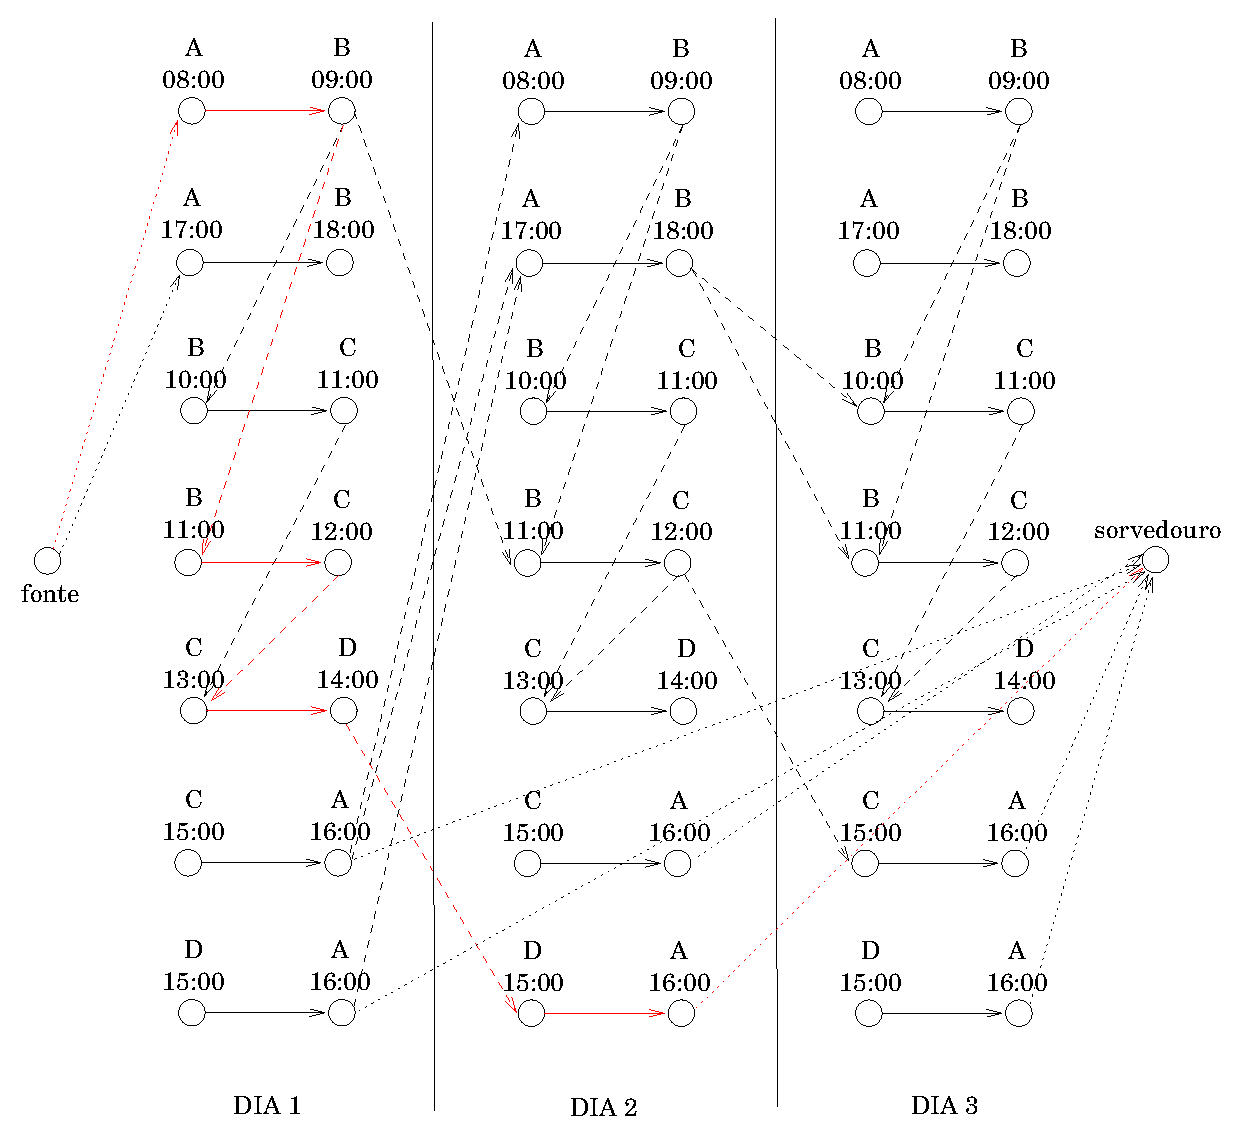
\includegraphics[scale=0.65]{fig/rede.eps}
		\caption{Rede de voos para a base $A$ de tripulantes. Arcos tracejados representam conexões 
		legais entre etapas. O caminho em vermelho representa uma das viagens possíveis.}
		\label{fig:rede}
	\end{center}
\end{figure}

%%%%%%%%%%%%%%%%%%%%%%%%%%%%%%%%%%%%%%%%%%%%%%%%%%%%%%%%%%%%%%%%%%%%%%%%%%%%%%%%%%%%%%%%%%%%%%%%%%%%

\subsection{Problema da Determinação de Escalas}
\label{sec:escalas}

No problema da determinação de escalas (ou, de forma mais restrita, problema da atribuição de
viagens), tem-se como entrada o conjunto de viagens obtido na resolução do PDV na etapa anterior, um
conjunto de atividades extra-voo, as regras utilizadas para confecção de escalas legais e,
finalmente, o conjunto de tripulantes para o qual se deseja gerar as escalas. A saída será uma
escala legal obtida para cada tripulante do conjunto considerado, tal que todas as atividades sejam
atribuídas o número de vezes necessário, e tal que o custo total da solução seja minimizado. Uma
esquema para entrada e saída do problema é apresentado na Figura~\ref{fig:pde}. Uma descrição 
detalhada sobre o problema pode ser encontrada em~\cite{kohl04}.

\begin{figure}[htbp]
	\begin{center}
		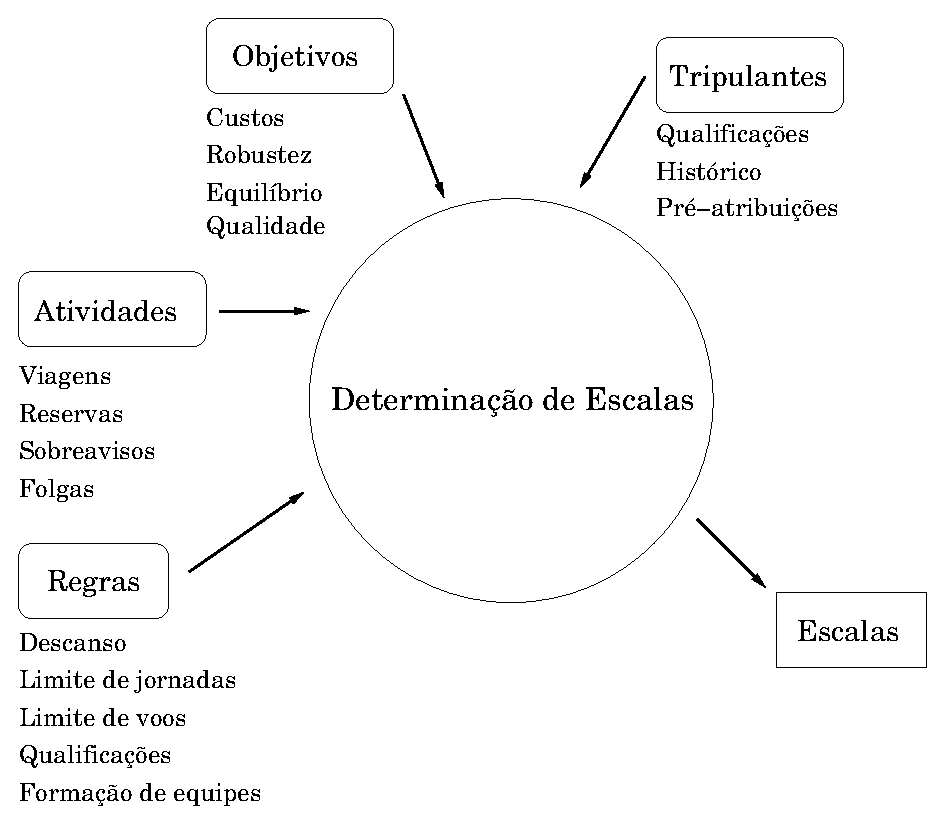
\includegraphics[scale=0.5]{fig/pde.eps}
		\caption{Representação do problema da determinação de escalas (PDE). Adaptado de~\cite{kohl04}.} 
		\label{fig:pde}
	\end{center}
\end{figure}

Nos dados de entrada são fornecidos os registros pessoais de cada tripulante, que incluem suas
qualificações, atividades pré-atribuídas, férias, etc. As qualificações contém informações, por
exemplo, sobre os equipamentos nos quais o tripulante está habilitado, ou sobre destinos onde ele
não pode operar devido a alguma restrição operacional. Atividades pré-atribuídas podem ser
folgas pedidas, exames médico, cursos, etc. Os registros de um tripulante também incluem atributos
acumulados, como o total de horas de voo realizadas durante o ano corrente. Outros dados de
interesse são, por exemplo, datas limites para treinamentos.

Outro conjunto de dados de entrada é formado pelas atividades a serem cobertas, que consiste das
viagens, reservas, sobreavisos, folgas, atividades de treinamento (\eg, treinamento em simulador e
cursos) e atividades em solo (\eg, exames médico). Normalmente, na formulação mais restrita do
problema, apenas as viagens devem ser atribuídas de forma automatizada e otimizada. Todas as outras
atividades são atribuídas \emph{a priori}, individualmente para cada tripulante em dias
pré-determinados dentro do horizonte de tempo do planejamento.

As regras típicas para construção de uma escala legal incluem limites máximos para horas de voo e
jornadas de trabalho, número mínimo de folgas, número máximo de dias consecutivos de trabalho, etc
(confira Seção~\ref{sec:regras_e_custos}). Essas são conhecidas como \emph{regras horizontais} pois
se aplicam a escalas únicas, e não considerem as outras escalas geradas na solução. Outro conjunto
de regras, conhecidas por \emph{regras verticais}, aplicam-se à solução como um todo. Um exemplo
típico está na atribuição de uma atividade que necessita ser realizada por mais de um membro de uma
tripulação com a mesma função. Outros exemplos de regras verticais são casos do tipo ``deve voar
com'', ou ``não deve voar com''.
 
A função objetivo no PDE é muito dependente da política da empresa. Existem basicamente quatro 
tipos de objetivos que podem ser encontrados em um problema desse tipo. Normalmente as empresas
adotam alguma combinação desses objetivos, seja introduzindo uma função objetivo combinada, seja
introduzindo restrições globais para algum deles enquanto otimizando outros. Os objetivos referem-se
a redução de custos reais, robustez da solução, distribuição equilibrada de trabalho e ``qualidade
de vida'' oferecida.

Vamos agora considerar o problema da determinação de escalas em sua forma mais simples. Sejam dados
um conjunto de atividade $\calA$, de cardinalidade $m_\calA$, e um conjunto de tripulantes $\calC$,
de cardinalidade $m_\calC$. Desejamos obter um conjunto de escalas $\calR_k \subset \calA$ para cada
tripulante $k$, $1 \leq k \leq m_\calC$, que particiona $\calA$,
%
\begin{equation*}
	\calA = \calR_1 \cup \calR_2 \cup \cdots \cup \calR_{m_\calC} \ev
\end{equation*}
%
de forma a minimizar alguma função objetivo linear nos custos $c_k$ de cada escala.

Um grande número de escalas $R_j \subset \calA$ podem ser geradas para cada tripulante. Idealmente,
todas as escalas legais poderiam ser geradas, mas para o resultado seria um número enorme dada a 
natureza combinatória do problema. Depois da geração de $n$ escalas, um problema de particionamento 
é resolvido para selecionar a melhor combinação de escalas que minimizem o custo da função objetivo.

Seja $x_j \in \{0, 1\}$, $1 \leq j \leq n$, uma variável de decisão cujo valor é 1 se a escala
$\calR_j$ for escolhida na solução, e 0 caso contrário. Seja $c_j$, $1 \leq j \leq n$, o custo 
associado à escala $\calR_j$. Seja ainda $A$ a matriz $m \times n$, onde $m = m_\calC + m_\calA$, 
com coeficientes $a_{ij}$ definidos por
%
\begin{equation*}
	a_{ij} = \left\{
	\begin{array}{ll}
			1 \ev & \text{se a escala $j$ foi gerada para o tripulante $i$, $i = 1, \ldots, m_\calC$} \\
			1 \ev & \text{se a escala $j$ contém a atividade $i - m_\calC$, 
			$i = m_\calC + 1, \ldots, m$} \\
			0 \ev & \text{caso contrário}
	\end{array}
	\right.
\end{equation*}

Com essas definições, o PDE é formulado da seguinte forma:
%
\begin{eqnarray} \label{eq:sppe}
	\text{minimizar} && \displaystyle \sum_{j=1}^n c_j x_j \nonumber \\
	\text{sujeito à} && \displaystyle \sum_{j=1}^n a_{ij} x_j = 1 \ev \;\; i = 1, \ldots, m \\
	                 && x_j \in \{0, 1\} \ev \;\; j = 1, \ldots, n \ep \nonumber
\end{eqnarray} 
%
Note que para cada tripulante exatamente uma escala deve ser determinada e cada atividade deve ser
atribuída a exatamente uma escala.

Suponha, por exemplo, que para cada tripulante três escalas sejam geradas. Então $n = 3m_\calC$, 
e a matriz de restrições $A$ assume forma semelhante~a:

\begin{center}
	\scalebox{0.85} {
		\begin{tabular}{ccccc}
			\begin{tabular}{ccc}
				\hline 
				\multicolumn{3}{c}{Tripulante$_1$} \\ \hline
				$\calR_1$ &	$\calR_2$ & $\calR_3$ \\ \hline
				1 & 1 & 1 \\
				0 & 0 & 0 \\
				$\vdots$ & $\vdots$ & $\vdots$ \\
				0 & 0 & 0 \\
				1 & 1 & 0 \\
				0 & 1 & 1 \\
				$\vdots$ & $\vdots$ & $\vdots$ \\
				1 & 0 & 1
			\end{tabular}
			& 
			\begin{tabular}{ccc}
				\hline 
				\multicolumn{3}{c}{Tripulante$_2$} \\ \hline
				$\calR_4$ &	$\calR_5$ & $\calR_6$ \\ \hline
				0 & 0 & 0 \\
				1 & 1 & 1 \\
				$\vdots$ & $\vdots$ & $\vdots$ \\
				0 & 0 & 0 \\
				1 & 0 & 1 \\
				0 & 0 & 1 \\
				$\vdots$ & $\vdots$ & $\vdots$ \\
				0 & 0 & 0
			\end{tabular}	
			& 
			\hspace{-0.3cm}
			\begin{tabular}{c}
				$\cdots$ \\
				$\cdots$ \\
				$\cdots$ \\
				$\cdots$ \\
				$\ddots$ \\
				$\cdots$ \\
				$\cdots$ \\
				$\cdots$ \\
				$\ddots$ \\
				$\cdots$
			\end{tabular}
			\hspace{-0.3cm}
			& 
			\begin{tabular}{ccc}
				\hline 
				\multicolumn{3}{c}{Tripulante$_{|\calC|}$} \\ \hline
				$\calR_{n-2}$ &	$\calR_{n-1}$ & $\calR_n$ \\ \hline
				0 & 0 & 0 \\
				0 & 0 & 0 \\
				$\vdots$ & $\vdots$ & $\vdots$ \\
				1 & 1 & 1 \\
				0 & 1 & 0 \\
				1 & 0 & 1 \\
				$\vdots$ & $\vdots$ & $\vdots$ \\
				0 & 1 & 0
			\end{tabular}	
			&
			\hspace{-0.3cm}
			\begin{tabular}{ccc}
				& & \\
				& & \\
				= & 1 & Atribuições \\
				= & 1 & \\
				$\vdots$ & $\vdots$ & \\
				= & 1 & \\
				= & 1 & Atividades \\
				= & 1 & \\
				$\vdots$ & $\vdots$ & \\
				= & 1 & 				
			\end{tabular} 
		\end{tabular}
	}
\end{center}

Existem dois tipos de restrições representadas pela matriz $A$ no modelo básico. As \emph{restrições 
de atribuições} garantem que todo tripulante tenha exatamente uma escala atribuída. Elas formam 
o primeiro bloco $m_\calC \times n$ de $A$. As \emph{restrições de atividades} garantem que cada 
atividade será atribuída exatamente uma vez na solução, formando o bloco final $m_\calA \times n$ 
final da matriz $A$.

Assim como no PDV, a formulação exposta acima do PDE apresenta dificuldade de resolução devido ao
número excessivo de variáveis e restrições. Mesmo os otimizadores mais potentes não são capazes de
resolver instâncias práticas do problemas em tempo viável. A solução é utilizar algum tipo de
heurística que encontre uma resposta sub-ótima para o problema, ou técnicas de otimização mais
avançadas como a geração implícita de colunas.

%%%%%%%%%%%%%%%%%%%%%%%%%%%%%%%%%%%%%%%%%%%%%%%%%%%%%%%%%%%%%%%%%%%%%%%%%%%%%%%%%%%%%%%%%%%%%%%%%%%%

\subsection{Formulação Integrada}
\label{sec:integrado}

Atualmente o PDV e o PDE são eficientemente tratados por uma série de técnicas que garantem soluções
próximas do ótimo com um tempo de processamento aceitável. Sistemas comerciais foram desenvolvidos
em torno dessas técnicas, sendo diariamente utilizados na maioria das empresas para resolução de
seus problemas de escalonamento~\cite{gopalakrishnan05}.

Um problema muito mais complexo seria o da integração entre o PDV e PDE, onde esses dois
sub-problemas seriam analisados e resolvidos simultaneamente. A vantagem dessa abordagem é motivada
pelos fatos descritos a seguir.

Primeiro, a fatoração do problema não permite que se estime adequadamente o custo
real de um escalonamento global. De fato, na determinação das viagens, busca-se minimizar o custo
associado à baixa produtividade de uma jornada de trabalho. Entretanto, o custo real do planejamento
só pode ser calculado após a atribuição das viagens aos tripulantes, ou seja, depois da solução do
PDE. Isso porque, para um dado horizonte de tempo, faz-se o pagamento de um salário fixo e mais 
um valor adicional para as horas excedentes.

Segundo, o conjunto ``ótimo de viagens'' provido na solução do PDV é determinado sem considerar o
número e a disponibilidade dos diferentes tripulantes. É claro que se pode incorporar no modelo as
restrições de bases (\ref{eq:bases}), mas elas fornecem apenas uma estimativa da mão de obra
disponível, pois não consideram as restrições impostas pelas regras que limitam a geração de escalas
legais. Na realidade, a disponibilidade real só é considerada enquanto se resolve o problema da
determinação de escalas.

A tendência recente nos trabalhos sobre escalonamento de tripulantes é de lidar com a versão
integrada do problema~\cite{saddoune12, souai09}, que apontam para ganhos econômicos da ordem de 5\%
com relação a versão sequencial. O problema completo, entretanto, é de difícil resolução, dado a
combinação do número de variáveis que já eram grandes no PDV e no PDE. Reporta-se
em~\cite{saddoune12} longos tempos de processamento mesmo para instâncias pequenas utilizando
técnicas de geração de colunas e agregação dinâmica de restrições. Uma alternativa interessante é a
utilização de meta-heurísticas como o algoritmo genético aplicado em~\cite{souai09}.

%%%%%%%%%%%%%%%%%%%%%%%%%%%%%%%%%%%%%%%%%%%%%%%%%%%%%%%%%%%%%%%%%%%%%%%%%%%%%%%%%%%%%%%%%%%%%%%%%%%%

\zerar
\section{Métodos de Solução para o PDV}
\label{sec:metodos}

O problema da determinação de viagens pode ser resolvido através de métodos exatos ou (meta)
heurísticos. A seguir discorreremos sobre cada um dos métodos estudados e utilizados neste trabalho.

%%%%%%%%%%%%%%%%%%%%%%%%%%%%%%%%%%%%%%%%%%%%%%%%%%%%%%%%%%%%%%%%%%%%%%%%%%%%%%%%%%%%%%%%%%%%%%%%%%%%

\subsection{Métodos Exatos}
\label{sec:metodos_exatos}

Os métodos exatos buscam a solução ótima global através de técnicas de otimização que resolvem o
problema de programação linear inteiro associado.

%%%%%%%%%%%%%%%%%%%%%%%%%%%%%%%%%%%%%%%%%%%%%%%%%%%%%%%%%%%%%%%%%%%%%%%%%%%%%%%%%%%%%%%%%%%%%%%%%%%%

\subsubsection{Set Partition}
\label{sec:metodos_partition}

No modelo {\it set partition} o problema é formulado de acordo com (\ref{eq:sppv}). A resolução pelo
otimizador é feita inicialmente considerando uma versão relaxada do problema, \ie, permitindo que as
variáveis $x_j$ assumam valores reais entre 0 e 1. A seguir, o problema relaxado é resolvido pelo
método Simplex, o que gera uma solução ótima fracionária $x^\ast$. A partir de $x^\ast$,
empregando-se um esquema {\it branch-and-bound}, obtém-se a melhor solução inteira. Vale ressaltar
que o procedimento {\it branch-and-bound} consome tempo e memória exponencial no número de
variáveis.

Observe que o modelo (\ref{eq:sppv}) não admite a existência de {\it deadheading}, \ie, tripulação 
viajando como passageiro, o que pode implicar a inviabilidade do problema.

%%%%%%%%%%%%%%%%%%%%%%%%%%%%%%%%%%%%%%%%%%%%%%%%%%%%%%%%%%%%%%%%%%%%%%%%%%%%%%%%%%%%%%%%%%%%%%%%%%%%

\subsubsection{Set Cover}
\label{sec:metodos_cover}

O modelo {\it set cover} é bastante similar ao {\it set partition}, porém admite a ocorrência de 
{\it deadheading} na solução final, possibilitando a viabilidade do problema.

As restrições adotadas no modelo {\it set cover} são dadas por (\ref{eq:dh}), onde permite-se que 
uma etapa seja coberta mais do que uma vez. Sendo $m$ o número de etapas a serem cobertas, podemos 
adicionar $m$ variáveis artificiais inteiras $y_i$, $i = 1, \ldots, m$, onde $y_i$ representa o 
número de vezes que a etapa $i$ é coberta como {\it deadhead}. Considerando um custo $d_i$ cada vez 
que a etapa $i$ é utilizada como {\it deadhead}, o problema de programação linear resultante é
%
\begin{eqnarray} \label{eq:scpdv}
	\text{minimizar} && \displaystyle \sum_{j=1}^n c_j x_j + \sum_{i=1}^m d_i y_i \nonumber \\
	\text{sujeito à} && \displaystyle \sum_{j=1}^n a_{ij} x_j - y_i = 1 \ev \;\; i = 1, \ldots, m \\
	                 && x_j \in \{0, 1\} \ev \;\; j = 1, \ldots, n \nonumber \\
	                 && y_i \geq 0 \ev \;\; i = 1, \ldots, m \ep \nonumber
\end{eqnarray}

O problema (\ref{eq:scpdv}) é resolvido pelo otimizador através dos mesmos procedimentos utilizados 
na resolução do {\it set cover} (Simplex e {\it branch-and-bound}). 

%%%%%%%%%%%%%%%%%%%%%%%%%%%%%%%%%%%%%%%%%%%%%%%%%%%%%%%%%%%%%%%%%%%%%%%%%%%%%%%%%%%%%%%%%%%%%%%%%%%%

\subsubsection{Geração de Colunas}
\label{sec:metodos_colunas}

Nesta seção descreveremos o método de geração de colunas para obtenção de uma solução ótima 
associada ao problema em (\ref{eq:scpdv}), chamado de problema mestre.

A ideia básica consiste em não gerar explicitamente todas as $n$ viagens possíveis do problema. 
Ao invés disso, começamos com um número reduzido de colunas que forneça ao menos uma solução viável
(o chamado problema restrito). Essas variáveis são levadas ao otimizador considerando a versão 
relaxada de (\ref{eq:scpdv}). Para determinar se o problema original com todas as $n$ variáveis 
está resolvido otimamente, solucionamos o seguinte subproblema:
%
\begin{equation} \label{eq:sub}
	w^\ast = \min_{j = 1, \ldots, n} \left[ c_j - \sum_{i=1}^m \pi_i a_{ij} \right] \ev
\end{equation} 
%
onde $\pi_i$, $i = 1, \ldots, m$ são as variáveis duais ótimas associadas ao problema restrito.
Da teoria da programação linear, sabemos que se $w^\ast \geq 0$ então o problema restrito é ótimo
ao problema mestre. Por outro lado, se  $w^\ast < 0$, a coluna $k$ (com custo reduzido 
$\bar{c}_k < 0$) é identificada e é adicionada ao problema restrito. O problema restrito é 
resolvido novamente e o processo se repete até que nenhuma variável de custo reduzido negativo 
seja encontrada.

Ocorre que o subproblema (\ref{eq:sub}) pode ser traduzido como um problema de caminho mais curto 
no grafo da rede de voos, o qual pode ser resolvido de forma eficiente. Mostraremos isso com mais 
detalhes na próxima versão deste trabalho.

%%%%%%%%%%%%%%%%%%%%%%%%%%%%%%%%%%%%%%%%%%%%%%%%%%%%%%%%%%%%%%%%%%%%%%%%%%%%%%%%%%%%%%%%%%%%%%%%%%%%

\subsection{Métodos (Meta) Heurísticos}
\label{sec:metodos_heuristicas}

%%%%%%%%%%%%%%%%%%%%%%%%%%%%%%%%%%%%%%%%%%%%%%%%%%%%%%%%%%%%%%%%%%%%%%%%%%%%%%%%%%%%%%%%%%%%%%%%%%%%

\subsubsection{Busca Local}
\label{sec:metodos_busca}

O método de busca local é bastante simples e foi um dos primeiros a ser utilizado na tentativa de 
melhorar uma solução viável do problema (\ref{eq:scpdv}). 

A busca local consiste em escolher aleatoriamente duas ou três viagens da solução viável inicial e, 
a partir da lista de etapas cobertas por essas viagens, gerar explicitamente todas as possíveis 
viagens legais usando o gerador. Como o número de etapas não é muito grande, o número de variáveis 
geradas é gerenciável. O modelo (\ref{eq:scpdv}) é então resolvido para todas essas variáveis, 
obtendo um novo conjunto de viagens que cobre o lista de etapas inicial. 

Se o custo desse novo conjunto de viagens for menor do que o original, então as viagens originais
serão substituídas na solução global. O processo é iterado um número máximo de vezes (ou um tempo 
máximo de execução), ou até que não haja variação significativa do custo (mínimo local), de tal 
forma que o custo sempre seja reduzido a cada passo.

%%%%%%%%%%%%%%%%%%%%%%%%%%%%%%%%%%%%%%%%%%%%%%%%%%%%%%%%%%%%%%%%%%%%%%%%%%%%%%%%%%%%%%%%%%%%%%%%%%%%

\subsubsection{Algoritmo Genético}
\label{sec:metodos_genetico}

Daremos aqui a formulação de um algoritmo genético para o problema (\ref{eq:scpdv}). 

%%%%%%%%%%%%%%%%%%%%%%%%%%%%%%%%%%%%%%%%%%%%%%%%%%%%%%%%%%%%%%%%%%%%%%%%%%%%%%%%%%%%%%%%%%%%%%%%%%%%

\zerar
\section{Resultados Obtidos}
\label{sec:resultados}

Em nosso estudo, utilizamos os pacotes de otimização GLPK (GNU Linear Programming Kit) e Cplex da
IBM. Os resultados finais, entretanto, são baseados apenas na utilização da ferramenta Cplex, uma
vez que a mesma provou ser mais eficiente. Além disso, o otimizador Cplex pôde ser utilizado
diretamente a partir de nosso código, alimentando o modelo gerado através da API Java fornecida pela
IBM. Por outro lado, como o GLPK não fornece API apropriada, sua utilização se limitou a geração do
modelo em arquivo (formato mps) e posterior execução do otimizador em um processo separado, sendo
necessário realizer um {\it parsing} no arquivo de saída gerado para obtenção dos resultados.

Restringimos o nosso estudo de escalonamento à resolução do problema de determinação de viagens.
Implementamos os métodos de solução do PDV descritos na Seção~\ref{sec:metodos}. Os parâmetros 
utilizados, que garantem a legalidade das viagens geradas, são apresentados na 
Tabela~\ref{tab:parametros} e baseiam-se na legislação brasileira para aviação comercial regular. 

Todos os testes foram realizados em um computador utilizando um processador Intel Core~i3 64~bits, 
com 4~Gb de memória RAM, rodando o sistema operacional MacOS~10.6. Toda a implementação foi escrita 
em Java (JDK~1.6.33).

\begin{table}
	\begin{center}
		\begin{tabular}{|l|l|l|}
			\hline 
			\bf Parâmetro & \bf Descrição & \bf Valor \\
			\hline \hline 
			\verb|MAX_LEGS| & Máximo de pernas por jornada & 5 \\ \hline
			\verb|MAX_FLIGHT_TIME| & Total máximo de voo por jornada & 9,5 h \\ \hline
			\verb|MAX_DUTY_TIME| & Duração máxima de uma jornada & 11,5 h \\ \hline
			\verb|MIN_SIT_TIME| & Tempo mínimo de conexão & 30 min \\ \hline
			\verb|MAX_SIT_TIME| & Tempo máximo de conexão & 120 min \\ \hline
			\verb|BRIEFING_TIME| & Tempo para o {\it briefing} & 0 min \\ \hline
			\verb|DEBRIEFING_TIME| & Tempo para o {\it debriefing} & 0 min \\ \hline
			\verb|MIN_REST_TIME| & Tempo mínimo de repouso & 12 h \\ \hline
			\verb|MAX_REST_TIME| & Tempo máximo de repouso & 36 h \\ \hline
			\verb|MAX_DUTIES| & Máximo de jornadas por viagem & 2, 3 ou 4 \\ \hline
			\end{tabular} 
			\caption{Parâmetros utilizados na geração das viagens.}
			\label{tab:parametros}
	\end{center}
\end{table}

%%%%%%%%%%%%%%%%%%%%%%%%%%%%%%%%%%%%%%%%%%%%%%%%%%%%%%%%%%%%%%%%%%%%%%%%%%%%%%%%%%%%%%%%%%%%%%%%%%%%

\subsection{Análise Preliminar}
\label{sec:analise_p}

O objetivo desta análise preliminar foi definir o limite de utilização do procedimento de geração
de viagens e do otimizador na resolução exata do modelo {\it set partition} (\ref{eq:sppv}).
Com essa finalidade, construímos alguns gráficos que relacionam o tempo de geração e otimiazação 
utilizado em nossa implementação, em função do número de etapas dadas como entrada do problema.

Para estudar a influência do número de pernas isoladamente, restringimos a entrada apenas para um
conjunto de voos entre duas localidades, São Paulo (CGH) e Rio de Janeiro (SDU), considerando os
trechos diárias oferecidos na ponte-aérea pela companhia aérea Gol. Um total de 62 pernas 
(31 de CGH para SDU e 31 de SDU para CGH) representam a instância global de entrada.

Vale observar que o caso da ponte-aérea é um pouco atípico no sentido de que representa um malha 
muito densa de voos: muitas etapas são oferecidas de ida e volta num curto intervalo de tempo, 
criando muitas conexões legais (arcos) entre os nós da rede de voos gerada. Com isso, o número
de viagens dado pela procedimento de busca no grafo explode rapidamente.

O gráfico da Figura~\ref{fig:pairings} mostra o número de viagens geradas em função do número de
etapas na ponte-aérea. As viagens foram geradas para a base CGH. São apresentadas três curvas, uma
para cada valor do parâmetro \verb|MAX_DUTIES| (2, 3 e 4). Observe a escala logarítmica do eixo
vertical. O comportamento praticamente linear das curvas indica um crescimento exponencial do número
de viagens que podem ser geradas. Observe ainda que a taxa de crescimento é maior quanto maior o
número máximo de jornadas permitidas, já que nesse caso permite-se um número muito maior de
combinações. Para \verb|MAX_DUTIES| = 4, encontrou-se um número da ordem de $10^8$ viagens com
apenas 36 pernas.

\begin{figure}[htp]
	\begin{center}
		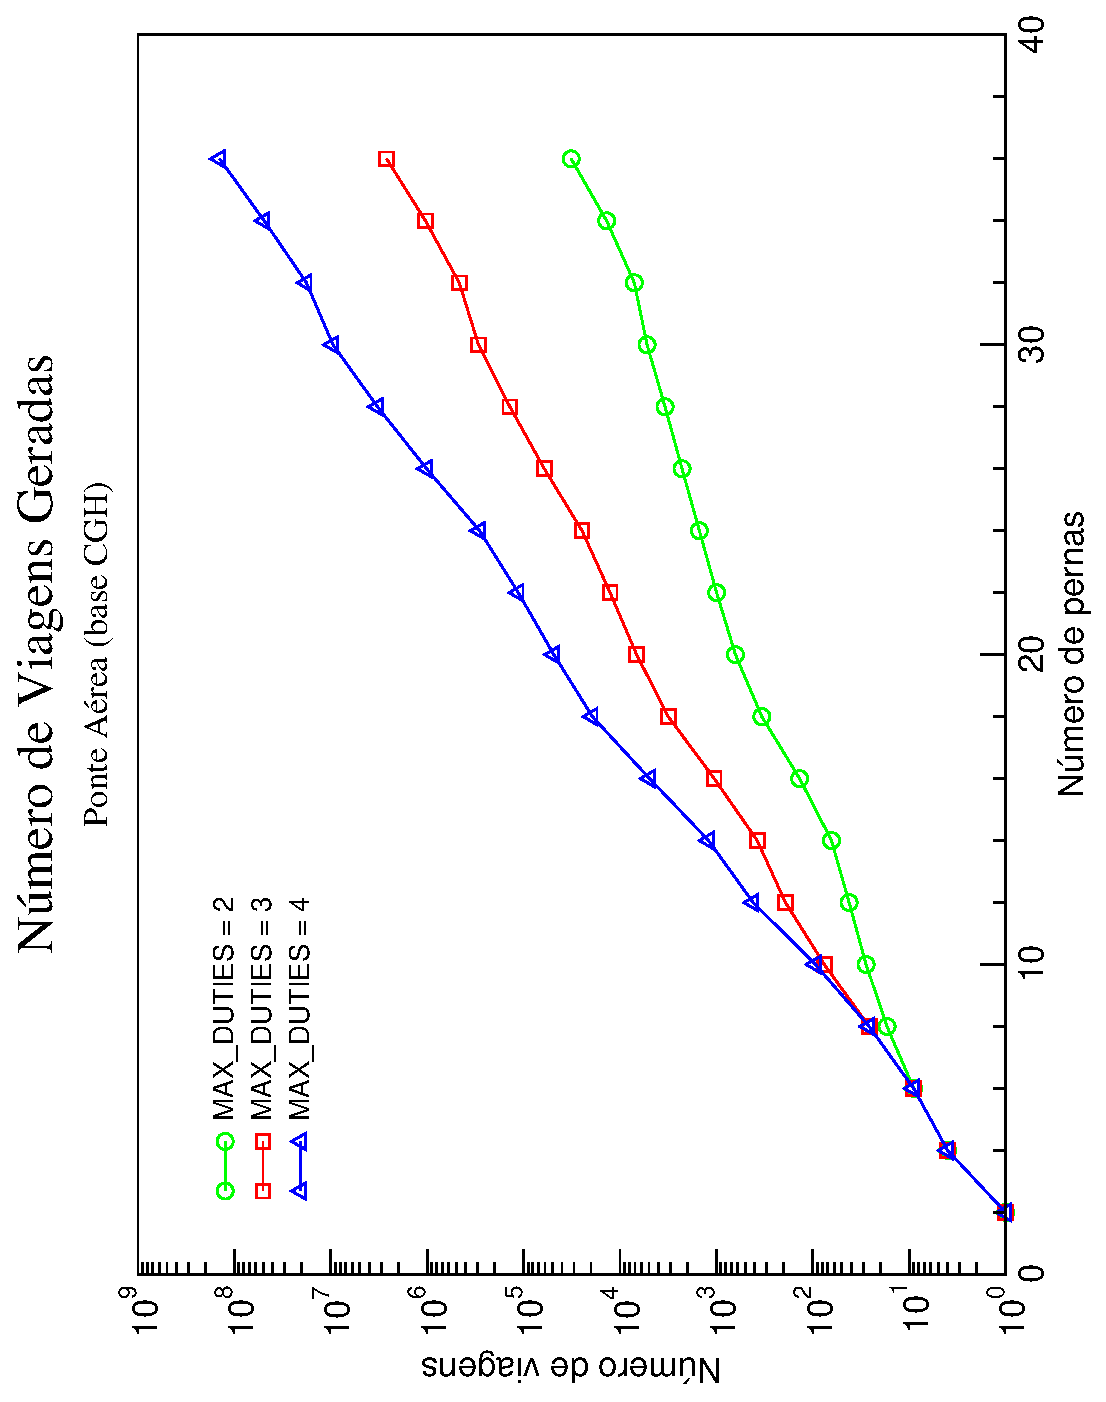
\includegraphics[scale=0.45,angle=-90]{fig/number_of_pairings.eps}
		\caption{Número de viagens geradas em função do número de pernas utilizadas na construção da
		rede de voos.}
		\label{fig:pairings}
	\end{center}
\end{figure}

O consumo de tempo gasto pelo algoritmo de busca em profundidade também foi medido em função do 
número de pernas. Os resultados são apresentados na Figura~\ref{fig:generation}. O comportamento das
curvas indicam também um crescimento exponencial do tempo gasto pelo algoritmo, ainda que ele seja
executado de forma rápida (para \verb|MAX_DUTIES| = 4, encontrou-se um tempos da ordem de $10^4$~ms 
para 36 pernas).

\begin{figure}[htb]
	\begin{center}
		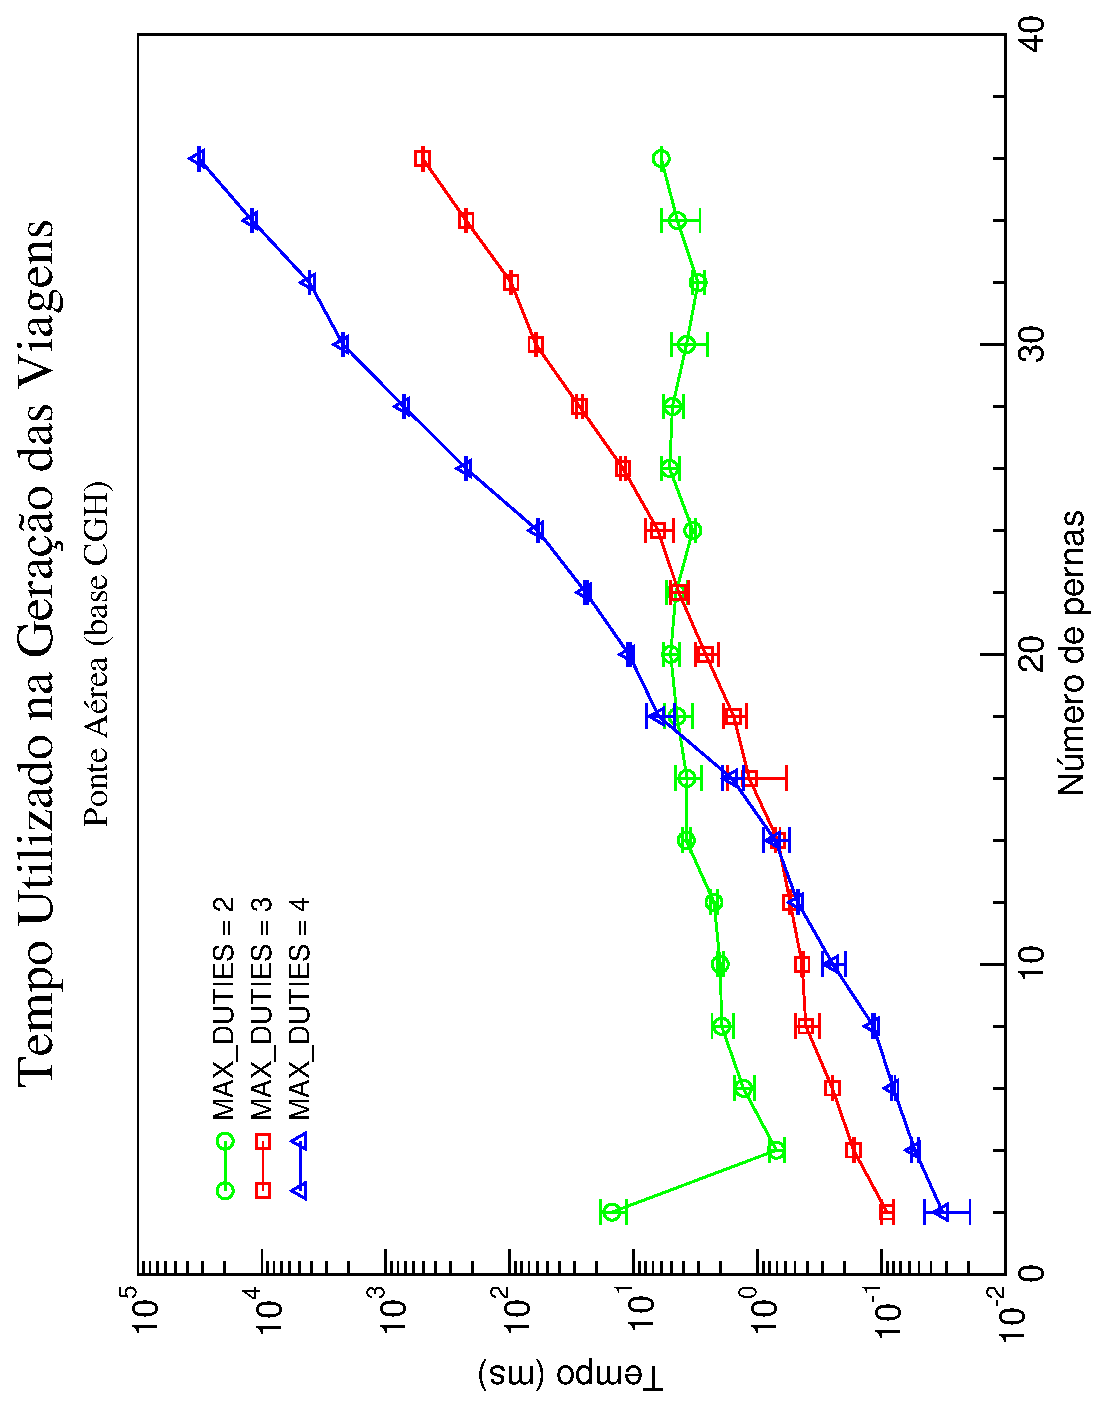
\includegraphics[scale=0.45,angle=-90]{fig/generation_time.eps}
		\caption{Tempo gasto na geração das viagens em função do número de pernas utilizadas na 
		construção da rede de voos. São apresentados valor médio $\pm$ desvio-padrão, considerando 5 
		medidas para cada ponto. O primeiro ponto da curva verde encontra-se um pouco fora provavelmente
		devido a algum transiente da máquina, visto que ele foi o primeiro a ser processado.}
		\label{fig:generation}
	\end{center}
\end{figure}

O tempo gasto pelo otimizador GLPK para resolver o modelo proposto é apresentado no gráfico da 
Figura~\ref{fig:glpk}. Mais uma vez, observa-se um crescimento exponencial muito forte (note a 
escala logarítmica do eixo vertical) em função do número de etapas considerado. A 
Figura~\ref{fig:cplex} mostra os resultados obtidos para o otimizador Cplex. 

\begin{figure}[htb]
	\begin{center}
		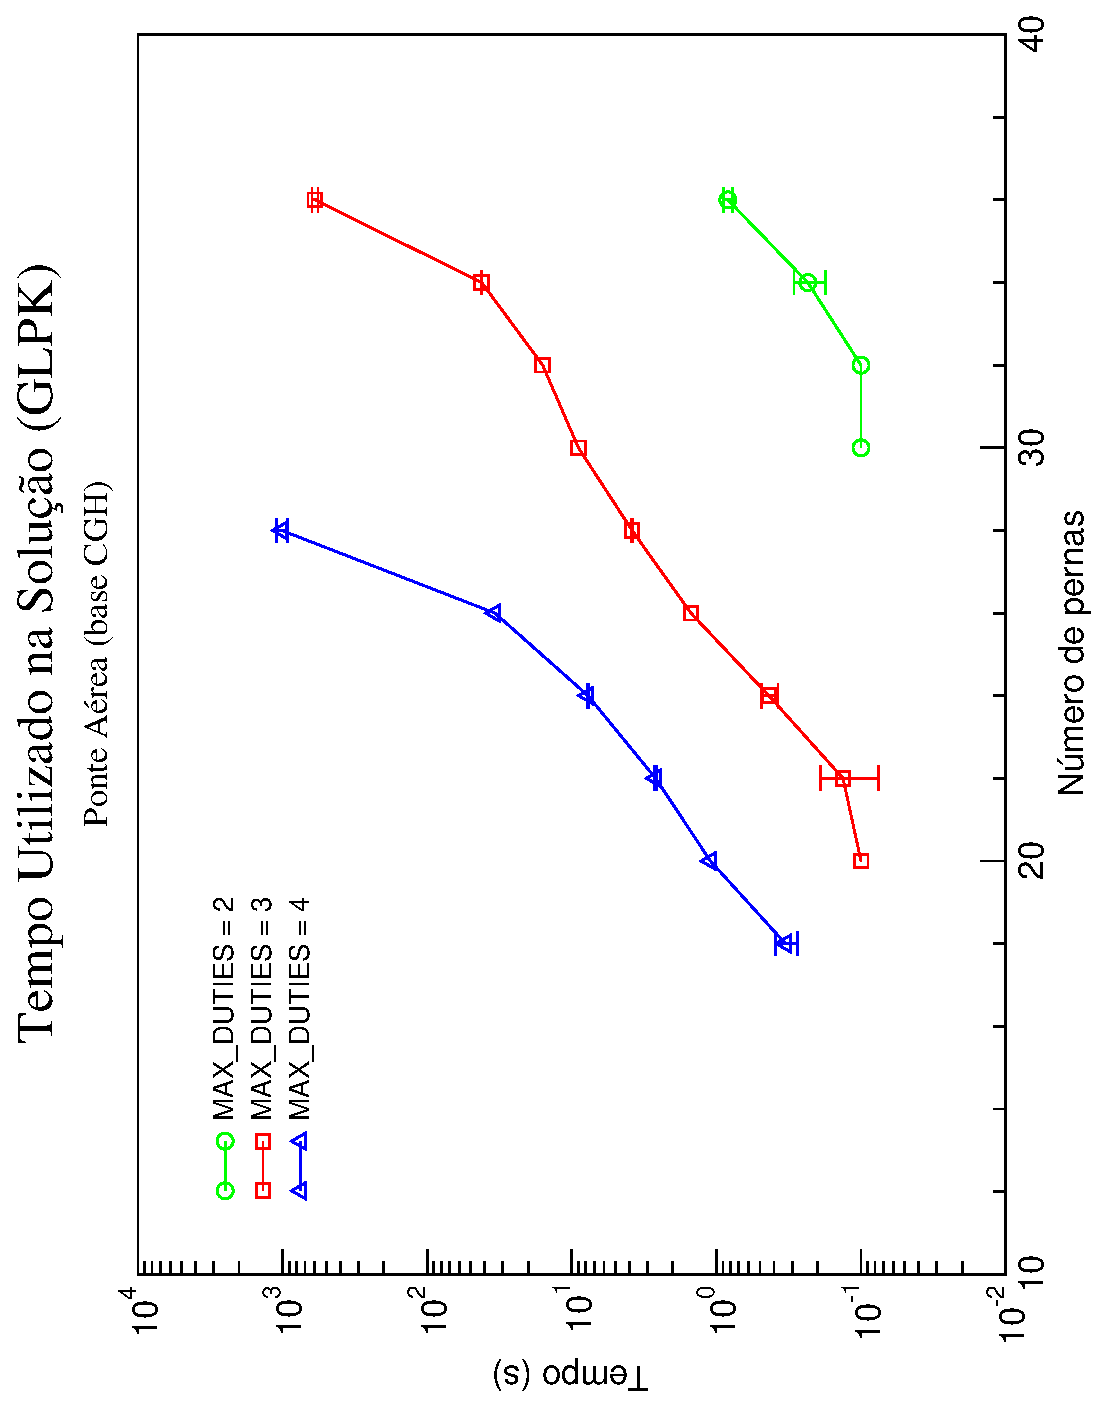
\includegraphics[scale=0.45,angle=-90]{fig/glpk_solution_time.eps}
		\caption{Tempo utilizado pelo otimizador GLPK na obtenção de uma solução inteira, em função do 
		número de etapas. São apresentados valor médio $\pm$ desvio-padrão, considerando 3 medidas para 
		cada ponto. Valores medidos com tempo de execução de 0,0~s não são apresentados (número pequeno 
		de pernas). Os últimos pontos da curva azul não puderam ser estimados, mesmo após algumas horas 
		de processamento.}
		\label{fig:glpk}
	\end{center}
\end{figure}

\begin{figure}[htb]
	\begin{center}
		\includegraphics[scale=0.45,angle=0]{fig/cplex_solution_time.eps}
		\caption{Resultados obtidos para o otimizador Cplex. Valem as mesmas observações feitas na 
		legenda da Figura~\ref{fig:glpk}.}
		\label{fig:cplex}
	\end{center}
\end{figure}

%%%%%%%%%%%%%%%%%%%%%%%%%%%%%%%%%%%%%%%%%%%%%%%%%%%%%%%%%%%%%%%%%%%%%%%%%%%%%%%%%%%%%%%%%%%%%%%%%%%%

\subsection{Métodos Exatos}
\label{sec:resultados_exatos}

Apenas três instâncias (pequenas) puderam ser resolvidas exatamente pela solução do modelo {\it set
partition} (\ref{eq:sppv}), com um tempo de processamento pequeno. A descrição das instâncias é
apresentada na Tabela~\ref{tab:instancias}, as quais foram extraídas de dados reais fornecidos por
companhias aéreas brasileiras. Na tabela são indicados o nome da instância, a companhia a qual
pertence, a frota de aeronaves (ou parte dela) a que se refere, as bases domiciliares dos
tripulantes, o número de etapas e o número de trilhos. O trilho identifica o conjunto de etapas que
uma determinada aeronave da frota deve executar diariamente. No caso de uma frota com $k$ aeronaves,
deverão ser fornecidos $k$ trilhos distintos.

\begin{table}[htb]
	\begin{center} 
		\begin{tabular}{|l|l|l|l|l|l|}
			\hline 
			{\bf Instância} & {\bf Cia} & {\bf Frota} & {\bf Bases} & {\bf Etapas} & {\bf Trilhos} \\ 
			\hline \hline
			73H\_26 & Gol & 737-800 & GRU & 26 & 5 \\ 
			738\_48 & WebJet & 737-800 & GRU GIG & 48 & 7 \\ 
			733\_92 & WebJet & 737-300 & GRU GIG POA & 92 & 12 \\ \hline
		\end{tabular}
		\caption{Caracterização das instâncias resolvidas exatamente através dos modelos 
		{\it set partition} e {\it set cover}. GRU = São Paulo, GIG = Rio de Janeiro e 
		POA = Porto Alegre.}
		\label{tab:instancias}
	\end{center}
\end{table}

Na resolução dos problemas, foram utilizados os parâmetros da Tabela~\ref{tab:parametros}. Além
disso, limitou-se a 1 o número máximo de trocas de aeronaves por jornada. Com isso, forçamos a
tripulação acompanhar, na medida do possível, o trilho percorrido pela aeronave, reduzindo a
possibilidade de conexões em cada localidade. Naturalmente os tempos de conexão serão reduzidos,
tornando as viagens geradas mais baratas e diminuindo o número total de variáveis geradas. Além
disso, esse procedimento torna a solução mais robusta, uma vez que o atraso de uma aeronave não
acarretará atraso na saída de outro voo que dependa daquela aeronave na troca.

O custo de uma viagem foi calculado como sendo o tempo ``ocioso'' relativo no qual o tripulante está 
trabalhando mas não está voando, ou seja, pela diferença entre o tempo total de uma viagem, menos o 
tempo total de voo efetuado, descontando ainda os tempos mínimos regulamentares de conexão entre 
pernas e de descanso entre jornadas, dividido pelo tempo total de voo. Esse custo avalia de forma 
relativa a produtividade de uma viagem, o qual deve ser minimizado na solução final.

Os resultados obtidos são apresentados e resumidos na Tabela~\ref{tab:resultados}. Nela são 
indicadas a instância resolvida, o número total de variáveis geradas, o número de viagens na 
solução, o custo da solução e o tempo de processamento do otimizador (Cplex).

\begin{table}[htb]
	\begin{center} 
		\begin{tabular}{|c|c|c|c|c|}
			\hline 
			{\bf Instância} & {\bf Variáveis} & {\bf Viagens} & {\bf Custo} & {\bf Tempo (s)} \\ 
			\hline \hline
			73H\_26 & 180 & 6 & 6,952 & $< 1$ \\ 
			738\_48 & 66411 & 6 & 6,436 & 3,75 \\
			733\_92 & 1023818 & 11 & 6,942 & 170,86 \\ \hline
		\end{tabular}
		\caption{Resultados obtidos na geração e otimização de viagens para as instâncias consideradas.}
		\label{tab:resultados}
	\end{center}
\end{table}

As mesmas instâncias 73H\_26, 738\_48, 733\_92 também foram resolvidas utilizando o modelo 
{\it set cover}, o qual admite a existência de {\it deadheading}. Os resultados obtidos foram 
idênticos aos listados na Tabela~\ref{tab:resultados}. Em particular, todas as variáveis 
artificiais $y_i$ receberam valor zero na solução final, indicando a não necessidade de 
{\it deadheading}.

%%%%%%%%%%%%%%%%%%%%%%%%%%%%%%%%%%%%%%%%%%%%%%%%%%%%%%%%%%%%%%%%%%%%%%%%%%%%%%%%%%%%%%%%%%%%%%%%%%%%

\subsubsection{Resultado Explícito}
\label{sec:resultado_explicito}

Para tornar mais concreto a entrada e a saída do problema, apresentamos na Tabela~\ref{tab:73H_26} o
conjunto de etapas referentes a instância 73H\_26\footnote{Não há problema de confidencialidade nos
dados apresentados.}. A mesma representa 26 trechos oferecidos diariamente pela companhia aérea Gol
para uma frota especial de 5 aeronaves B737-800. Para cada etapa são fornecidos o seu número,
aeroporto de origem, aeroporto de destino, horário local de decolagem (DEP) e horário local de pouso
(ARR) e o trilho correspondente.

Na Tabela~\ref{tab:pairings} listamos as 6 viagens geradas como solução do problema de otimização.
Cada etapa na tabela apresenta o número do voo, origem e destino, horário local de decolagem e 
pouso, e o trilho executado. O custo final resultante foi de 6,952, para um total de 180 variáveis 
geradas, considerando a base GRU (São Paulo). Observe a presença de uma viagem bate-volta (4),
bem como uma viagem de 3 dias de duração (5).

\begin{table}[!htb]
	\begin{center}
		\begin{tabular}{|cccccc|}
			\hline 
			{\bf Número} & {\bf Origem} & {\bf Destido} & {\bf DEP} & {\bf ARR} & {\bf Trilho} \\
			\hline \hline
			7625 & GRU &	GIG	 &  07:00	 &  08:00  & 1 \\
			7622 & GIG &	GRU	 &  09:00	 &  09:55	 & 1 \\
			7622 & GRU &	CCS	 &  11:00	 &  15:30	 & 1 \\
			7622 & CCS &	AUA	 &  16:10	 &  17:55	 & 1 \\
			7623 & AUA &	CCS	 &  21:20	 &  22:05	 & 1 \\
			7623 & CCS &	GRU	 &  22:45	 &  06:00	 & 1 \\
			1841 & CWB &	GRU	 &  07:52	 &  08:55	 & 2 \\
			1902 & GRU &	NAT	 &  11:00	 &  14:20	 & 2 \\
			1903 & NAT &	GRU	 &  15:30	 &  19:10	 & 2 \\
			1704 & GRU &	MAO	 &  21:15	 &  00:10	 & 2 \\
			1798 & GRU &	REC	 &  08:05	 &  11:21	 & 3 \\
			1149 & REC &	GRU	 &  12:04	 &  15:30	 & 3 \\
			7680 & GRU &	AEP	 &  18:25	 &  21:15	 & 3 \\
			7681 & AEP &	GRU	 &  22:40	 &  01:30	 & 3 \\
			1705 & MAO &	GRU	 &  03:42	 &  08:35	 & 4 \\
			1766 & GRU &	CWB	 &  09:20	 &  10:16	 & 4 \\
			1846 & CWB &	GRU	 &  11:13	 &  12:15	 & 4 \\
			7480 & GRU &	ASU	 &  13:05	 &  13:50	 & 4 \\
			1847 & GRU &	CWB	 &  18:10	 &  19:20	 & 4 \\
			1767 & CWB &	GRU	 &  20:56	 &  21:50	 & 4 \\
			1566 & GRU &	CWB	 &  22:35	 &  23:30	 & 4 \\
			7481 & ASU &	GRU	 &  14:30	 &  17:25	 & 4 \\
			7678 & GRU &	AEP	 &  08:00	 &  10:50	 & 5 \\
			7679 & AEP &	GRU	 &  11:50	 &  14:35	 & 5 \\
			7658 & GRU &	EZE	 &  15:15	 &  18:15	 & 5 \\
			7659 & EZE &	GRU	 &  20:35	 &  23:25	 & 5 \\ \hline
	\end{tabular}
	\caption{Dados de entrada da instância 73H\_26, contendo 26 etapas e 5 trilhos.}
	\label{tab:73H_26}
	\end{center}
\end{table}

\begin{table}[!htb]
	\begin{center}
		\begin{tabular}{|c|c|ccccc|}
			\hline
			{\bf Viagem} & {\bf Jornada} & \multicolumn{5}{|c|}{\bf Etapa} \\ \hline \hline
			\multirow{6}{*}{1} & \multirow{4}{*}{1}  
			  & 7625 & GRU-GIG & 07:00 & 08:00 & 001 \\
			& & 7622 & GIG-GRU & 09:00 & 09:55 & 001 \\
			& & 7622 & GRU-CCS & 11:00 & 15:30 & 001 \\
			& & 7622 & CCS-AUA & 16:10 & 17:55 & 001 \\ \cline{2-7}
			                       & \multirow{2}{*}{2}
				& 7623 & AUA-CCS & 21:20 & 22:05 & 001 \\
			& &	7623 & CCS-GRU & 22:45 & 06:00 & 001 \\ \hline \hline
			\multirow{2}{*}{2} & \multirow{2}{*}{1}  		
				& 1902 & GRU-NAT & 11:00 & 14:20 & 002 \\
			& & 1903 & NAT-GRU & 15:30 & 19:10 & 002 \\ \hline \hline
			\multirow{2}{*}{3} & \multirow{1}{*}{1}  		
				& 1704 & GRU-MAO & 21:15 & 00:10 & 002 \\ \cline{2-7}
                           	& \multirow{1}{*}{2}
				&	1705 & MAO-GRU & 03:42 & 08:35 & 004 \\ \hline \hline
			\multirow{2}{*}{4} & \multirow{2}{*}{1}  		
				& 1798 & GRU-REC & 08:05 & 11:21 & 003 \\
			& & 1149 & REC-GRU & 12:04 & 15:30 & 003 \\ \hline \hline			
			\multirow{10}{*}{5} & \multirow{3}{*}{1}  
				&	1847 & GRU-CWB & 18:10 & 19:20 & 004 \\
			& &	1767 & CWB-GRU & 20:56 & 21:50 & 004 \\
			& &	1566 & GRU-CWB & 22:35 & 23:30 & 004 \\ \cline{2-7}
                           		& \multirow{4}{*}{2}
				&	1841 & CWB-GRU & 07:52 & 08:55 & 002 \\
			&	&	1766 & GRU-CWB & 09:20 & 10:16 & 004 \\
			&	&	1846 & CWB-GRU & 11:13 & 12:15 & 004 \\
			&	&	7480 & GRU-ASU & 13:05 & 13:50 & 004 \\ \cline{2-7}
                           		& \multirow{3}{*}{3}
				&	7481 & ASU-GRU & 14:30 & 17:25 & 004 \\
			&	&	7680 & GRU-AEP & 18:25 & 21:15 & 003 \\
			&	&	7681 & AEP-GRU & 22:40 & 01:30 & 003 \\ \hline \hline
			\multirow{4}{*}{6} & \multirow{3}{*}{1}  
				& 7678 & GRU-AEP & 08:00 & 10:50 & 005 \\
			& & 7679 & AEP-GRU & 11:50 & 14:35 & 005 \\
			&	& 7658 & GRU-EZE & 15:15 & 18:15 & 005 \\ \cline{2-7}
                           	 & \multirow{1}{*}{2}
				& 7659 & EZE-GRU & 20:35 & 23:25 & 005 \\ \hline
		\end{tabular}
		\caption{Conjunto de viagens obtido como solução ótima da instância 73H\_26.}
		\label{tab:pairings}
	\end{center}
\end{table}
			                               
%%%%%%%%%%%%%%%%%%%%%%%%%%%%%%%%%%%%%%%%%%%%%%%%%%%%%%%%%%%%%%%%%%%%%%%%%%%%%%%%%%%%%%%%%%%%%%%%%%%%

\subsection{Métodos (Meta) Heurísticos}
\label{sec:resultados_heuristicas}

%%%%%%%%%%%%%%%%%%%%%%%%%%%%%%%%%%%%%%%%%%%%%%%%%%%%%%%%%%%%%%%%%%%%%%%%%%%%%%%%%%%%%%%%%%%%%%%%%%%%

\subsubsection{Busca Local}
\label{sec:resultados_busca}

Após a implementação mostraremos os resultados obtidos pelo método da busca local para as instâncias 
maiores do problema, com alguns gráficos do custo em função do número de iterações, para diversas 
escolhas dos parâmetros do algoritmo. 

A ideia também é aplicar o método para as instâncias que puderam ser resolvidas otimamente, com o 
intuito de se avaliar o quão perto do ótimo o método pode ser capaz de chegar nesses casos.

%%%%%%%%%%%%%%%%%%%%%%%%%%%%%%%%%%%%%%%%%%%%%%%%%%%%%%%%%%%%%%%%%%%%%%%%%%%%%%%%%%%%%%%%%%%%%%%%%%%%

\subsubsection{Algoritmo Genético}
\label{sec:resultados_genetico}

Após a implementação mostraremos os resultados obtidos pelo método da busca local para as instâncias 
maiores do problema, com alguns gráficos do custo em função do número de iterações, para diversas 
escolhas dos parâmetros do algoritmo. Faremos também a comparação com o método da busca local.

%%%%%%%%%%%%%%%%%%%%%%%%%%%%%%%%%%%%%%%%%%%%%%%%%%%%%%%%%%%%%%%%%%%%%%%%%%%%%%%%%%%%%%%%%%%%%%%%%%%%

\zerar
\section{Conclusões}
\label{sec:conclusoes}

Com relação a análise preliminar apresentada na Seção~\ref{sec:analise_p}, concluímos que o
procedimento de geração de viagens leva a um número gigantesco de variáveis, mesmo para um pequeno
número de pernas (Figura~\ref{fig:pairings}). Isso porque a natureza combinatória do problema leva o
algoritmo de busca a explorar diversas possibilidades, principalmente em uma rede como a da ponte
aérea, onde existem diversas possibilidades de conexão toda vez que se chega em uma das localidades.
Além disso, essas possibilidades se multiplicam quando consideramos um maior número de jornadas
permitidas (\verb|MAX_DUTIES|). Apesar disso, a geração de viagens ainda se fez em tempo aceitável,
podendo ser aplicada para redes maiores (Figura~\ref{fig:generation}).

Entretanto, quando esse número enorme de variáveis é levado ao otimizador, o tempo de processamento
se torna impraticável. Para se certificar disso, basta extrapolar as curvas obtidas nas
Figuras~\ref{fig:glpk} e~\ref{fig:cplex}. {\bf Uma tentativa de resolução de uma instância da
ponte-aérea contendo 40 etapas, não pode ser resolvida mesmo após 12 horas de processamento.} Ainda
assim, ficamos surpresos com a capacidade do otimizador resolver instâncias com um número de
variáveis da ordem de $10^6$ em tempo aceitável (resultados da Tabela~\ref{tab:resultados}).

A análise preliminar então nos mostra que o método de ``gerar-e-otimizar'' para resolver o modelo
(\ref{eq:sppv}) não é adequado para resolver o problema de forma geral. Em particular, das milhares
de variáveis geradas, apenas poucas delas são escolhidas para entrar na solução final, como se pode
observar da Tabela~\ref{tab:resultados}. Isso indica que o procedimento de geração explícita de 
variáveis não é adequado, pois muitas delas não servem para nada. Um procedimento mais inteligente
seria o de gerar apenas variáveis ``boas'', ou seja, com grande chance de aparecerem na solução 
final. O método de geração de colunas desenvolve essa ideia e será explorado futuramente.

Com relação aos resultados obtidos utilizando o modelo {\it set cover}, observamos que como as 
colunas associadas às variáveis $y_i$ de {\it deadheading} (reveja o formulação (\ref{eq:scpdv})) 
foram ajustadas com preços altos, e como os problemas analisados eram viáveis do ponto de vista do 
{\it set partition}, o otimizador conseguiu encontrar as mesmas soluções obitidas sem a presença de 
{\it deadheading}. Concluímos que a utilização de {\it deadheading} só será realizada se for 
estritamente necessária para viabilidade do problema.

%%%%%%%%%%%%%%%%%%%%%%%%%%%%%%%%%%%%%%%%%%%%%%%%%%%%%%%%%%%%%%%%%%%%%%%%%%%%%%%%%%%%%%%%%%%%%%%%%%%%

% Bibliografia BiBTeX
\bibliography{../bib/crew_scheduling}
\bibliographystyle{plain}
 
\end{document}

